\chapter{Giới thiệu}
\section{Bài toán và sản phẩm}
Project xây dựng GlucoGuide, một ứng dụng web tích hợp hai nhánh xử lý của sơ đồ học phần. Nhánh dữ liệu sử dụng mô hình mạng nơ-ron nhiều lớp để phân loại nhãn nguy cơ tổng hợp và dự đoán điểm tiến triển bệnh trong dữ liệu nghiên cứu. Nhánh tri thức kế thừa kho tài liệu của tiểu luận 02, tổ chức các khái niệm cùng quan hệ trên Neo4j và truy xuất văn bản theo câu hỏi. Kết quả hai nhánh được trình bày cùng nguồn bằng chứng và nhật ký xử lý.

GlucoGuide phát triển từ các thực nghiệm học phần, bổ sung cơ chế phối hợp giữa mô hình, truy xuất và phản hồi. Toàn bộ kết quả đánh giá được lưu cùng mã nguồn để thuận tiện đối chiếu.
\section{Phạm vi đầu ra}
Hai bộ dữ liệu có định nghĩa nhãn khác nhau. Bộ phân loại gồm các nhãn High, Moderate và Low của dữ liệu tổng hợp. Bộ hồi quy gồm những người đã mắc bệnh và một thước đo tiến triển sau một năm. Vì vậy không thể ghép một nhãn High với một điểm hồi quy để suy ra xác suất mắc bệnh. Ứng dụng dùng hai biểu mẫu riêng và công bố phạm vi ngay tại đầu ra.

Bản công khai sử dụng tổng hợp trích đoạn xác định. Câu trả lời được ghép từ các đoạn văn truy xuất được và thông tin về phạm vi mô hình; không gọi mô hình ngôn ngữ bên ngoài. Bản cục bộ dùng Qwen3 4B lượng tử hóa để diễn đạt trên tài liệu truy xuất; các yêu cầu có nguy cơ được phân loại trước và xử lý bằng luật. Hai chế độ đều phụ thuộc chất lượng và độ phủ của kho tài liệu.
\section{Mục tiêu đánh giá}
Phân loại được đo bằng accuracy và macro-F1. Hồi quy được đo bằng MAE và hệ số xác định. Truy xuất cần kiểm tra cả tài liệu được chọn và quan hệ có nguồn trên Neo4j. Kiểm tra ứng dụng tập trung vào các tình huống có bằng chứng, thiếu bằng chứng, thiếu đầu vào, giá trị không hợp lệ và cơ sở dữ liệu đồ thị không hoạt động.
\chapter{Agent và cơ chế phối hợp}
\section{Vai trò xử lý}
Hệ thống phân chia trách nhiệm thành an toàn, mô hình, truy xuất văn bản, đồ thị tri thức, chính sách trình bày, ngôn ngữ và kiểm chứng phản hồi. Các agent có handler được gọi qua MessageBus; nhật ký lưu người gửi, người nhận, loại thông điệp và nội dung. Các thành phần hoạt động trong một tiến trình FastAPI dưới điều phối tập trung, chưa phải các dịch vụ tự chủ độc lập.

Một thông điệp REQUEST thể hiện yêu cầu xử lý. INFORM ghi nhận kết quả và FAILURE thể hiện thành phần không thực hiện được. Khi Neo4j không hoạt động, hệ thống ghi FAILURE và chỉ dùng các đoạn văn cục bộ, không giả lập kết quả đồ thị. Khi thiếu đầu vào mô hình, hệ thống trả lại danh sách trường cần bổ sung trước khi suy luận.
\section{Reinforcement Learning kết hợp luật}
Chính sách được học trong môi trường mô phỏng luồng xử lý, không mô phỏng hiệu quả điều trị. Trạng thái gồm hai biến nhị phân: đã có kết quả mô hình và đã có bằng chứng truy xuất. Bốn trạng thái tương ứng với bốn tổ hợp của hai biến này. Ba hành động là hỏi làm rõ, trả lời có nguồn và giải thích mô hình kèm nguồn.

Hàm thưởng bằng một nếu hành động phù hợp trạng thái, bằng âm một trong trường hợp còn lại. Khi chưa có bằng chứng, hành động mục tiêu là hỏi làm rõ. Khi có bằng chứng nhưng chưa có kết quả mô hình, hành động mục tiêu là trả lời có nguồn. Khi có cả hai, hành động mục tiêu là giải thích mô hình và dẫn nguồn. Đây là hàm thưởng do người thiết kế quy định; không phải đánh giá của bệnh nhân hay chuyên gia.
\[
Q(s,a)\leftarrow Q(s,a)+\alpha[r-Q(s,a)].
\]
Mỗi episode kết thúc sau một hành động, nên không có thành phần bootstrap tương lai. Cấu hình gồm 3.000 episode, seed 254, tốc độ học 0,15 và xác suất khám phá 0,2. Vì bài toán chỉ có một bước, thí nghiệm minh họa cơ chế học giá trị hành động nhưng chưa chứng minh khả năng lập kế hoạch dài hạn. Luật thiếu bằng chứng luôn ép hành động hỏi làm rõ, kể cả khi chính sách học đề xuất hành động khác.
\section{Giới hạn của kiến trúc}
Mỗi agent có handler, bộ nhớ trong lượt và thông điệp yêu cầu/phản hồi có thể kiểm tra. Hệ thống chưa có bộ nhớ hội thoại bền vững, cơ chế tranh biện hoặc triển khai agent thành dịch vụ độc lập. Nhật ký nhiều vai trò giúp quan sát xử lý, nhưng không tự chứng minh mức tự chủ hoặc lợi ích so với một pipeline đơn giản hơn.
\chapter{Kiến trúc tổng quan}
\begin{figure}[htbp]\centering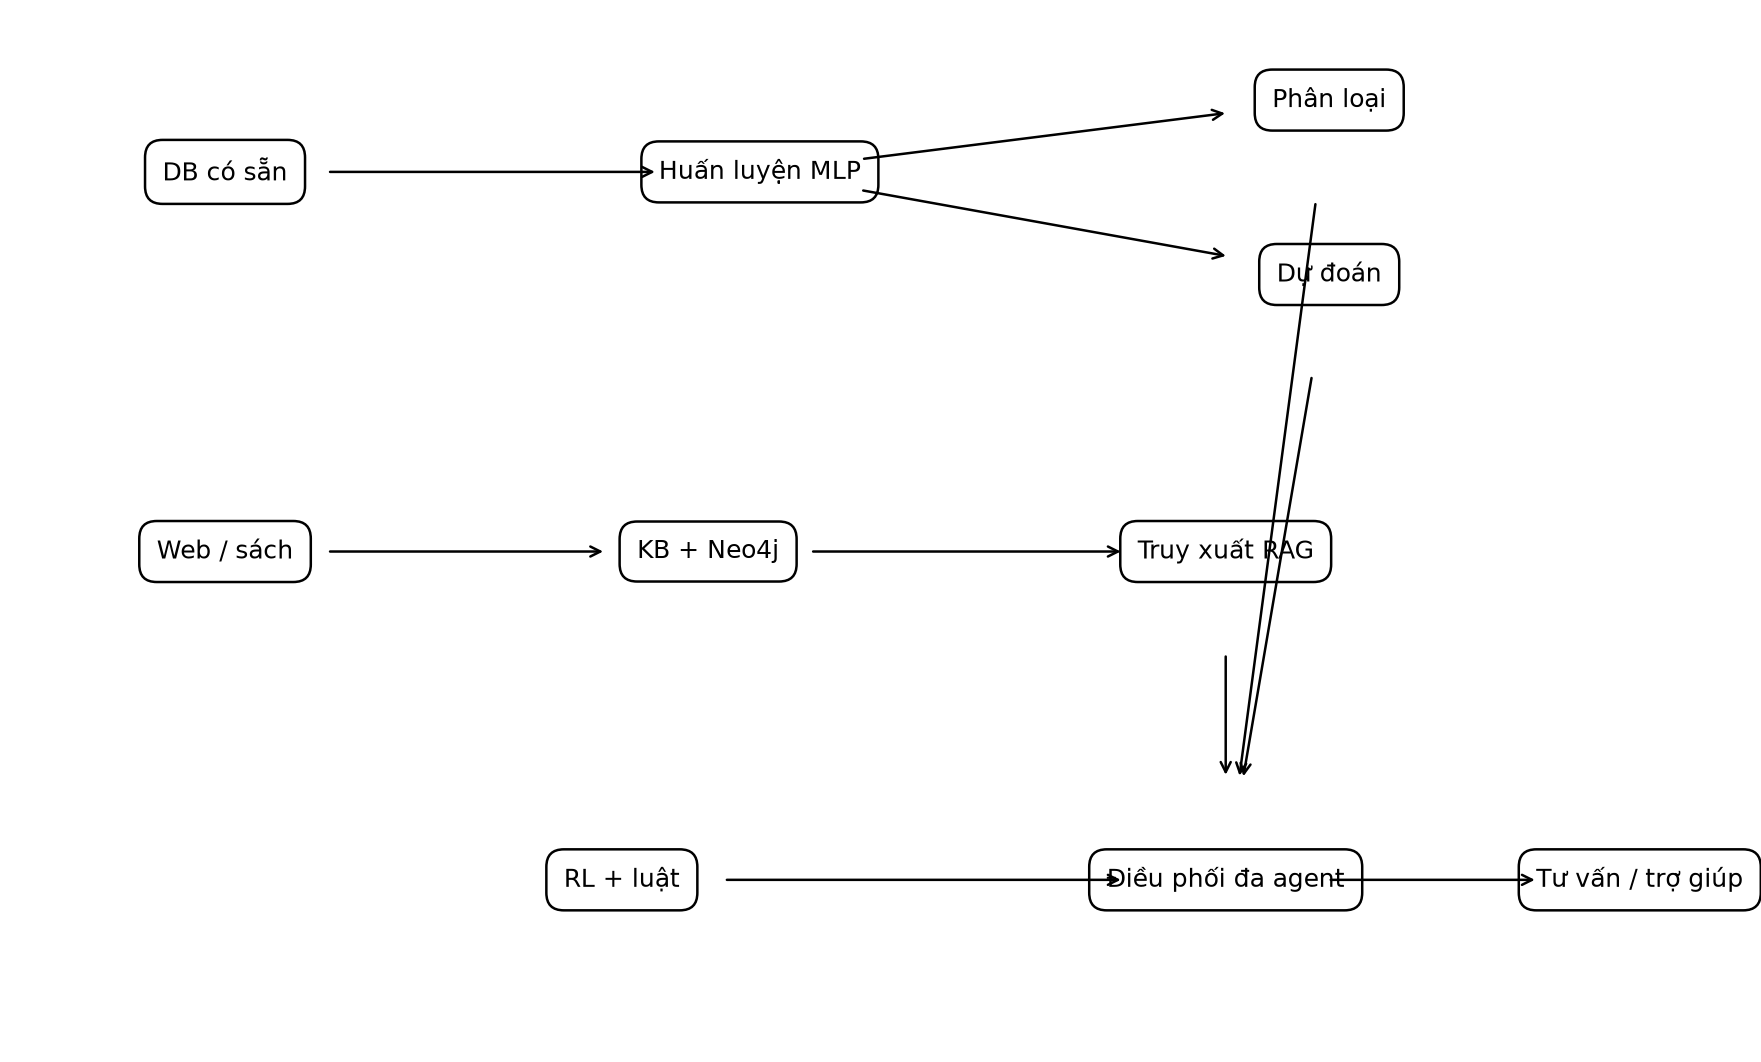
\includegraphics[width=\linewidth]{figures/architecture.png}\caption{Hai nhánh hội tụ về điều phối và trợ giúp, dựng lại từ sơ đồ trên bảng.}\end{figure}
\section{Nhánh dữ liệu}
DB có sẵn cung cấp dữ liệu cho quá trình huấn luyện. Pipeline phân loại gồm điền trung vị, chuẩn hóa và MLP. Pipeline hồi quy chuẩn hóa dữ liệu rồi suy luận bằng MLP. Hai đầu ra đều đi tới vùng phản hồi của ứng dụng. Trong lúc phục vụ, mô hình được nạp từ checkpoint; ứng dụng không huấn luyện lại theo câu hỏi của người dùng.
\section{Nhánh tri thức}
Nguồn tri thức là các đoạn văn đã được tổ chức trong tiểu luận 02. Mỗi tài liệu có mã, tiêu đề, từ khóa, văn bản, định danh nguồn và các bộ ba. Project bảo toàn những trường này khi chuyển sang kho tri thức mới. Việc cập nhật hướng dẫn y tế từ web chưa tự động hóa; phiên bản kho tài liệu phải được xem như một bản chụp dữ liệu cần rà soát trước khi mở rộng phạm vi sử dụng.

Kho tri thức gồm 58 đoạn từ 22 nguồn được tham chiếu. Mọi đoạn đều có quan hệ gắn với nguồn và trích đoạn làm căn cứ; tổng cộng 106 bộ ba được nạp vào Neo4j local. Nội dung gồm xét nghiệm, ăn uống, vận động, theo dõi, thuốc, các loại tiểu đường và trợ giúp sinh hoạt.

Một bộ ba gồm khái niệm đầu, tên quan hệ và khái niệm cuối. Neo4j lưu hai đầu dưới nhãn Concept; quan hệ RELATED\_TO có thuộc tính label biểu diễn tên quan hệ, document biểu diễn tài liệu và evidence biểu diễn đoạn văn làm căn cứ. Ràng buộc duy nhất theo tên khái niệm và thao tác MERGE giúp nạp lại dữ liệu mà không tạo các bản sao giống hệt.
\section{Luồng người dùng}
Yêu cầu được phân loại an toàn trước khi chuyển đến truy xuất. Yêu cầu mô hình phải đi qua kiểm tra các trường trước khi suy luận. Văn bản và kết quả đồ thị được chuyển sang đối chiếu; chính sách học và luật xác định kiểu phản hồi. Giao diện hiển thị câu trả lời, tài liệu nguồn và các bước xử lý. Lớp hội thoại nhận tối đa 64 thông điệp gần nhất để giải quyết câu hỏi tiếp nối; chỉ dùng câu hỏi người dùng làm gợi ý chủ đề, không dùng lời trả lời cũ làm căn cứ y tế. Các trường của hai mô hình được tách riêng để tránh biến đổi sai đơn vị hoặc tự suy diễn giá trị còn thiếu.

Sau khi chạy một trong hai mô hình, nút ``Nhận xét và hỗ trợ'' gửi lại loại bài toán và các giá trị đã nhập đến agent mô hình. Chatbot trả lời bằng nhãn hoặc điểm thực tế của mẫu, kèm chỉ số đánh giá ngoài mẫu và giới hạn sử dụng. Nhánh này dùng giải thích xác định, không để Qwen suy đoán ý nghĩa lâm sàng của nhãn tổng hợp hoặc điểm tiến triển.
\chapter{Nguồn dữ liệu và quy trình chuẩn bị}
\section{Phân biệt dữ liệu mô hình với tài liệu tri thức}
Project sử dụng hai bộ dữ liệu học có giám sát và một kho tài liệu. Bộ phân loại cung cấp nhãn High, Moderate, Low; bộ hồi quy cung cấp một điểm tiến triển sau một năm; KB cung cấp văn bản giải thích và nguồn. Ba thành phần này có mục tiêu khác nhau. Dữ liệu mô hình không tự trở thành hướng dẫn y khoa, còn tài liệu y khoa không được coi là nhãn huấn luyện cho hai MLP.

\begin{longtable}{p{3cm}p{4cm}p{7cm}}\caption{Danh mục dữ liệu thực sự dùng trong GlucoGuide.}\label{tab:datasets}\\\toprule Thành phần & Quy mô & Nơi lấy và nơi sử dụng\\\midrule\endfirsthead\toprule Thành phần & Quy mô & Nơi lấy và nơi sử dụng\\\midrule\endhead
Phân loại & 50.000 dòng, 41 cột gốc; dùng 8 biến & Kaggle, Diabetes Risk Prediction Dataset (50K patients), tài khoản mobeenfatimah. ZIP lưu tại \path{data/raw/diabetes.zip}; dùng trong \path{scripts/train_models.py}.\\
Hồi quy & 442 dòng, 10 biến và target số & Bộ diabetes đi kèm scikit-learn, đọc bằng \texttt{load\_diabetes(scaled=False)}. Không dùng ZIP của bài toán phân loại.\\
Tri thức & 21 đoạn; 9 nguồn đang được tham chiếu & \path{data/knowledge.json}; 20 đoạn kế thừa kho tiểu luận 02 và một đoạn mô tả phạm vi phân loại bổ sung. 32 bộ ba được nạp lên Neo4j.\\\bottomrule\end{longtable}
\section{Nguồn và phiên bản bộ phân loại}
Trang công bố bộ dữ liệu: \url{https://www.kaggle.com/datasets/mobeenfatimah/diabetes-risk-prediction-dataset-50k-patients}. Tệp nằm trong ZIP có tên \path{diabetes_risk_prediction_dataset.csv}. Báo cáo sử dụng đúng snapshot đã lưu trên máy, không tự thay bằng bộ 100.000 bản ghi của bài tham khảo. Tệp kiểm kê \path{results/data_audit.json} lưu SHA-256 của ZIP để phân biệt các phiên bản tải về.

Đơn vị quan sát là một bản ghi tổng hợp, không phải hồ sơ lâm sàng được project thu thập. Cột mục tiêu là \texttt{Diabetes\_Risk}. Kiểm kê trực tiếp thấy 36.593 nhãn High, 12.937 Moderate và 470 Low, tương ứng 73,186\%, 25,874\% và 0,94\%. Một mô hình chỉ đoán High sẽ có accuracy 73,186\% trên toàn bộ snapshot; vì vậy phải đọc accuracy cùng macro-F1 và recall từng lớp.

Không có nhãn thiếu và không có dòng trùng hoàn toàn trên 41 cột. Kết luận về dòng trùng không chứng minh các hồ sơ là những cá nhân độc lập, nhất là khi bảng có cột định danh. Pipeline hiện giữ nguyên 50.000 dòng, không có bước loại trùng hay loại ngoại lệ. Những đặc điểm này được công bố để người đọc biết chính xác dữ liệu nào đã đi vào phép chia.
\section{Từ điển đầu vào và giá trị thiếu}
\begin{longtable}{p{6cm}rp{5cm}}\caption{Kiểm kê tám biến đầu vào trên toàn bộ CSV, trước tiền xử lý.}\label{tab:data-fields}\\\toprule Biến & Số ô thiếu & Min / trung vị / max\\\midrule\endfirsthead\toprule Biến & Số ô thiếu & Min / trung vị / max\\\midrule\endhead
Age & 497 & 18 / 54 / 90\\
BMI & 0 & 11.9 / 30 / 61.7\\
HbA1c & 1974 & 4.5 / 8.5 / 12.5\\
Fasting\_Blood\_Sugar & 0 & 65 / 142.6 / 220\\
Blood\_Glucose & 959 & 70 / 159.9 / 250\\
Blood\_Pressure\_Systolic & 0 & 90 / 140 / 190\\
HDL & 1000 & 25 / 57.3 / 90\\
LDL & 1000 & 50 / 135.1 / 220\\\bottomrule\end{longtable}
Các cột được chọn lần lượt là tuổi, BMI, HbA1c, đường huyết lúc đói, glucose, huyết áp tâm thu, HDL và LDL. Min, trung vị, max ở Bảng~\ref{tab:data-fields} là thống kê mô tả của snapshot, không phải khoảng bình thường hay ngưỡng chẩn đoán. Trên giao diện, nút điền mẫu lấy đúng giá trị của bộ dữ liệu. Người dùng không nên tự thay một chỉ số ở đơn vị khác rồi coi kết quả tương đương.

Những trường \texttt{Patient\_ID}, \texttt{Diabetes\_Risk\_Score}, \texttt{AI\_Health\_Recommendation} và \texttt{Doctor\_Consultation\_Needed} không được chọn làm đặc trưng. Đặc biệt, điểm nguy cơ và khuyến nghị có thể gắn trực tiếp với quy trình tạo nhãn; đưa chúng vào dễ khiến bài toán trở thành khôi phục thông tin đã gần như có sẵn. Việc bỏ các trường này giảm một nguy cơ rò rỉ, nhưng không chứng minh mọi phụ thuộc trong dữ liệu tổng hợp đã được loại bỏ.

Trung vị dùng để điền thiếu được học trên tập train của pipeline, không dùng trung vị của toàn bộ bảng ở Bảng~\ref{tab:data-fields}. Sau đó StandardScaler học trung bình và độ lệch chuẩn trên train. Pipeline chứa cả imputer, scaler và mô hình được lưu bằng joblib, nhờ đó web dùng cùng phép biến đổi với quá trình huấn luyện. Khi nhập từ web, các trường hiện vẫn bắt buộc; imputer chủ yếu phục vụ giá trị thiếu trong dữ liệu huấn luyện và kiểm tra.
\section{Phép chia và dấu vết tái lập}
Phân loại chia 80/20, phân tầng theo nhãn, seed 254: 40.000 dòng train và 10.000 dòng test. Chỉ số dòng bắt đầu từ 0 và nhãn train/test được lưu tại \path{results/classification_split.csv}. Tập test có 7.319 High, 2.587 Moderate và 94 Low. Kiểm kê dữ liệu không huấn luyện lại mô hình và không thay kết quả đã báo cáo.

MLP bật early stopping với phần validation nội bộ của thư viện. Validation này nằm bên trong train ngoài, nhưng imputer và scaler đã fit trước khi MLP tách validation. Đây là điểm cần cải thiện nếu thiết kế một thí nghiệm chọn mô hình nghiêm ngặt. Test ngoài không được dùng để fit pipeline. Báo cáo không nhận rằng đã có ba tập train/validation/test tách trước toàn bộ tiền xử lý.
\section{Nguồn bộ hồi quy và ý nghĩa mục tiêu}
Nguồn phân phối: \url{https://scikit-learn.org/stable/modules/generated/sklearn.datasets.load_diabetes.html}. Nguồn gốc được thư viện dẫn tới nghiên cứu Least Angle Regression và trang dữ liệu thống kê: \url{https://www4.stat.ncsu.edu/~boos/var.select/diabetes.html}. Bộ dữ liệu gồm 442 người đã mắc bệnh với mục tiêu là một đại lượng tiến triển sau một năm; mô tả của thư viện không cho phép đổi mục tiêu đó thành đường huyết hoặc xác suất mắc bệnh\cite{diabetes}.

Project gọi \texttt{scaled=False}, sau đó chuẩn hóa bằng scaler của riêng train. Mười cột gồm age, sex, bmi, bp và s1 đến s6. age là tuổi, bmi là chỉ số khối cơ thể, bp là huyết áp trung bình. Theo metadata, s1 là cholesterol toàn phần, s2 LDL, s3 HDL, s4 tỷ lệ cholesterol/HDL, s5 được mô tả thận trọng là có thể là log triglyceride, s6 là chỉ số đường huyết. sex được giữ nguyên mã nghiên cứu; không dùng mã này để tự chọn ngưỡng y khoa.

Bộ hồi quy không có giá trị thiếu trong ma trận đặc trưng. Phép chia ngẫu nhiên seed 254 giữ 353 mẫu train và 89 mẫu test, ghi tại \path{results/regression_split.csv}. Hai mô hình cùng dùng phép chia này. Chỉ số dòng trong \path{results/regression_predictions.csv} cho phép truy lại mục tiêu thật và dự đoán của từng mẫu test.
\section{Nguồn KB và nguồn đang thực sự được dùng}
\begin{longtable}{p{5cm}p{8cm}r}\caption{Nguồn thực sự được 46 tài liệu trong KB tham chiếu.}\label{tab:kb-sources}\\\toprule Nguồn & Mã tài liệu & Số đoạn\\\midrule\endfirsthead\toprule Nguồn & Mã tài liệu & Số đoạn\\\midrule\endhead
NIDDK · Xét nghiệm \& chẩn đoán & a1c, testing & 2\\
CDC · Xử trí hạ đường huyết & low, urgent & 2\\
CDC · Lập kế hoạch bữa ăn & plate, carb, fruit, meal\_example, rice\_portion, fruit\_whole & 6\\
WHO · Diabetes & activity, symptoms, overview & 3\\
NIDDK · Quản lý bệnh tiểu đường & medicine, monitor, care\_questions, glucose\_log, new\_diagnosis & 5\\
scikit-learn · Dữ liệu diabetes & meanpressure, triglyceride, demographics, model & 4\\
AHA · Hiểu số đo huyết áp & bloodpressure & 1\\
MedlinePlus · Các chỉ số cholesterol & lipids, hdl, ldl, ratio & 4\\
Bộ dữ liệu tổng hợp Diabetes Risk Prediction 50K & classification\_scope & 1\\
NIDDK · Diabetes \& Foot Problems & foot\_care & 1\\
CDC · Managing Sick Days & sick\_day & 1\\
NIDDK · Quick Reference on UACR \& GFR & kidney\_checks & 1\\
CDC · Get Active & activity\_plan & 1\\
NIDDK · What Is Diabetes? & types\_compare, prediabetes, pregnancy\_diabetes, complications & 4\\
NIDDK · Healthy Living with Diabetes & drinks, meal\_timing, alcohol & 3\\
NIDDK · Insulin, Medicines \& Treatments & metformin\_info, insulin\_info, missed\_medicine & 3\\
CDC · Diabetes and Mental Health & diabetes\_distress, stress\_glucose & 2\\
ADA · Facts About Diabetes & not\_contagious & 1\\
ADA · Diabetes Remission Criteria & remission\_info & 1\\\bottomrule\end{longtable}\noindent\textbf{NIDDK · Xét nghiệm \& chẩn đoán}\par\noindent\url{https://www.niddk.nih.gov/health-information/diabetes/overview/tests-diagnosis}\par\medskip

\noindent\textbf{CDC · Xử trí hạ đường huyết}\par\noindent\url{https://www.cdc.gov/diabetes/treatment/treatment-low-blood-sugar-hypoglycemia.html}\par\medskip

\noindent\textbf{CDC · Lập kế hoạch bữa ăn}\par\noindent\url{https://www.cdc.gov/diabetes/healthy-eating/diabetes-meal-planning.html}\par\medskip

\noindent\textbf{WHO · Diabetes}\par\noindent\url{https://www.who.int/news-room/fact-sheets/detail/diabetes}\par\medskip

\noindent\textbf{NIDDK · Quản lý bệnh tiểu đường}\par\noindent\url{https://www.niddk.nih.gov/health-information/diabetes/overview/managing-diabetes}\par\medskip

\noindent\textbf{scikit-learn · Dữ liệu diabetes}\par\noindent\url{https://scikit-learn.org/stable/modules/generated/sklearn.datasets.load_diabetes.html}\par\medskip

\noindent\textbf{AHA · Hiểu số đo huyết áp}\par\noindent\url{https://www.heart.org/en/health-topics/high-blood-pressure/understanding-blood-pressure-readings}\par\medskip

\noindent\textbf{MedlinePlus · Các chỉ số cholesterol}\par\noindent\url{https://medlineplus.gov/cholesterollevelswhatyouneedtoknow.html}\par\medskip

\noindent\textbf{Bộ dữ liệu tổng hợp Diabetes Risk Prediction 50K}\par\noindent\url{https://www.kaggle.com/datasets/mobeenfatimah/diabetes-risk-prediction-dataset-50k-patients}\par\medskip

\noindent\textbf{NIDDK · Diabetes \& Foot Problems}\par\noindent\url{https://www.niddk.nih.gov/health-information/diabetes/overview/preventing-problems/foot-problems}\par\medskip

\noindent\textbf{CDC · Managing Sick Days}\par\noindent\url{https://www.cdc.gov/diabetes/living-with/managing-sick-days.html}\par\medskip

\noindent\textbf{NIDDK · Quick Reference on UACR \& GFR}\par\noindent\url{https://www.niddk.nih.gov/health-information/professionals/advanced-search/quick-reference-uacr-gfr}\par\medskip

\noindent\textbf{CDC · Get Active}\par\noindent\url{https://www.cdc.gov/diabetes/living-with/physical-activity.html}\par\medskip

\noindent\textbf{NIDDK · What Is Diabetes?}\par\noindent\url{https://www.niddk.nih.gov/health-information/diabetes/overview/what-is-diabetes}\par\medskip

\noindent\textbf{NIDDK · Healthy Living with Diabetes}\par\noindent\url{https://www.niddk.nih.gov/health-information/diabetes/overview/healthy-living-with-diabetes}\par\medskip

\noindent\textbf{NIDDK · Insulin, Medicines \& Treatments}\par\noindent\url{https://www.niddk.nih.gov/health-information/diabetes/overview/insulin-medicines-treatments}\par\medskip

\noindent\textbf{CDC · Diabetes and Mental Health}\par\noindent\url{https://www.cdc.gov/diabetes/living-with/mental-health.html}\par\medskip

\noindent\textbf{ADA · Facts About Diabetes}\par\noindent\url{https://diabetes.org/about-diabetes/diabetes-myths}\par\medskip

\noindent\textbf{ADA · Diabetes Remission Criteria}\par\noindent\url{https://diabetes.org/newsroom/international-experts-outline-diabetes-remission-diagnosis-criteria}\par\medskip
Danh mục sources trong JSON có 13 mục, nhưng chỉ 9 mục đang được tài liệu tham chiếu; không được ghi rằng cả 13 nguồn đều đóng góp vào phản hồi hiện tại. Mỗi đoạn có id, title, terms, text, source và triples. Các đoạn này là bản biên soạn ngắn kế thừa và mô tả kỹ thuật của project, không phải toàn văn sách hoặc bản tải tự động từ website.

Luồng Web/sách đến KB trong sơ đồ được hiện thực ở mức biên soạn snapshot có nguồn. Project chưa có nút upload PDF, trình thu thập web, cơ chế cập nhật định kỳ hay bộ chia chương sách tự động. Các PDF tham khảo của sinh viên chỉ phục vụ bố cục và phân tích thiết kế; chúng không được nạp làm nguồn tư vấn y khoa. Khi thay KB cần rà nội dung, cập nhật JSON, chạy lại script nạp Neo4j và khởi động lại backend để xây lại ma trận TF-IDF.

Hai mươi đoạn kế thừa chứa 32 bộ ba. Đoạn \texttt{classification\_scope} bổ sung giải thích nhãn tổng hợp và không có bộ ba, do đó số đoạn tăng lên 21 nhưng số cạnh vẫn là 32. Theo quy tắc MERGE hiện tại, các cạnh tạo 60 nút Concept. Các số đếm JSON là kiểm kê dữ liệu nguồn; số nút/cạnh trên web được lấy trực tiếp từ cơ sở dữ liệu để xác nhận nạp thành công.
\section{Từ nguồn tới kết quả hiển thị}
Đường đi phân loại là ZIP/CSV, chọn cột, chia dữ liệu, fit pipeline, lưu checkpoint, API và giao diện. Đường đi hồi quy là hàm tải của thư viện, chia dữ liệu, fit pipeline, checkpoint và API. Đường đi tri thức là đoạn văn có nguồn, chỉ mục TF-IDF và bộ ba Neo4j, lựa chọn bằng chứng rồi tổng hợp trích đoạn.

Các tệp \path{results/model_metrics.json}, \path{results/classification_predictions.csv}, \path{results/regression_predictions.csv} và \path{results/api_scenarios.json} lần lượt lưu số liệu tổng hợp, dự đoán chi tiết và kiểm thử chức năng. Script \path{scripts/audit_data.py} sinh bảng dữ liệu của báo cáo và bản danh mục dùng trên web từ cùng một snapshot. Tách thống kê dữ liệu, metric mô hình và kiểm thử API giúp tránh coi việc ứng dụng chạy thành công là bằng chứng mô hình dự đoán tốt.
\chapter{Các thành phần và thực nghiệm}
\section{Phân loại}
Dữ liệu tổng hợp gồm 50.000 dòng. Tám biến đầu vào là tuổi, BMI, HbA1c, đường huyết lúc đói, glucose, huyết áp tâm thu, HDL và LDL. Các biến chứa điểm nguy cơ, khuyến nghị sức khỏe và yêu cầu gặp bác sĩ không được đưa vào mô hình. Phép chia phân tầng với seed 254 giữ 40.000 dòng huấn luyện và 10.000 dòng kiểm tra.

MLP có ba tầng ẩn 64, 32 và 16 đơn vị, dừng sớm và tối đa 150 vòng lặp. Trung vị và tham số chuẩn hóa được học trên tập huấn luyện ngoài. Cơ chế early stopping của thư viện chia tiếp một phần dữ liệu cho validation; do tiền xử lý nằm trước MLP, các tham số tiền xử lý đã nhìn thấy phần validation nội bộ này. Tập test ngoài vẫn độc lập, nhưng để kiểm soát validation nghiêm ngặt hơn cần tách validation trước toàn bộ pipeline.

Logistic Regression dùng trọng số lớp cân bằng làm đối chứng. MLP dùng cấu hình mặc định không cân bằng trọng số. Vì hai cấu hình có cách xử lý mất cân bằng khác nhau, chênh lệch kết quả không chỉ phản ánh kiến trúc mạng. Accuracy cần đọc cùng macro-F1, đặc biệt với lớp Low hiếm.
\section{Hồi quy}
Bộ diabetes từ scikit-learn được tải ở dạng chưa chuẩn hóa, gồm 442 quan sát với 10 biến đầu vào. Phép chia seed 254 giữ 353 mẫu huấn luyện và 89 mẫu kiểm tra. Ridge với hệ số điều chuẩn 10 là đối chứng. MLP có ba tầng ẩn 64, 32 và 16, dừng sớm và tối đa 1.000 vòng lặp.

Các biến s1 đến s6 là những trường nghiên cứu của bộ dữ liệu. Không được thay tên hoặc đơn vị bằng suy đoán khi nhập hồ sơ ngoài đời. Mục tiêu của demo là minh họa quy trình suy luận từ mô hình đã lưu. Chất lượng trên bộ dữ liệu nhỏ không chứng minh khả năng chuyển sang quần thể Việt Nam.
\section{Kết quả kiểm tra}
\begin{table}[htbp]\centering\caption{Phân loại trên 10.000 mẫu kiểm tra.}\begin{tabular}{lrr}\toprule Mô hình & Accuracy & Macro-F1\\\midrule
Logistic Regression & 0.6965 & 0.5005\\
MLP & 0.8180 & 0.5441\\\bottomrule\end{tabular}\end{table}
\begin{table}[htbp]\centering\caption{Hồi quy trên 89 mẫu kiểm tra.}\begin{tabular}{lrr}\toprule Mô hình & MAE & $R^2$\\\midrule
Ridge & 44.0555 & 0.4791\\
MLP & 44.3225 & 0.4758\\\bottomrule\end{tabular}\end{table}

MLP cải thiện accuracy và macro-F1 so với Logistic Regression trong lần chạy này. Tuy nhiên macro-F1 còn thấp so với accuracy, phản ánh hiệu năng không đồng đều giữa các lớp. Ở hồi quy, Ridge có MAE thấp hơn và hệ số xác định cao hơn MLP. Báo cáo vẫn trình diễn MLP để minh họa nhánh Deep Learning, đồng thời công bố đầy đủ đối chứng và không nhận MLP là mô hình tốt nhất.
\section{Truy xuất và đồ thị}
Văn bản được chuẩn hóa không dấu rồi biểu diễn bằng TF--IDF từ và ký tự. Điểm kết hợp dùng trọng số 0,55 và 0,45, có cộng ưu tiên nhỏ cho từ khóa và chủ đề. Câu hỏi được biến đổi bằng cùng từ vựng. Điểm truy xuất là tích vô hướng của các vector đã chuẩn hóa. Hệ thống giữ tối đa bốn đoạn có điểm đạt ngưỡng 0,15 và ít nhất 58\% điểm của đoạn đứng đầu. Các ngưỡng là cấu hình triển khai, chưa được tối ưu trên một bộ validation độc lập.

Agent đồ thị lấy các cạnh có thuộc tính document trùng với mã tài liệu đã truy xuất, kiểm tra bộ ba, trích đoạn và URL rồi cấp quan hệ có nguồn vào ngữ cảnh Qwen. Đây là truy xuất văn bản kết hợp căn cứ đồ thị theo tài liệu, chưa phải bộ máy suy luận nhiều bước. Một nhãn quan hệ không chứng minh quan hệ nhân quả. Khi không có tài liệu đủ điểm, hệ thống yêu cầu làm rõ; khi Neo4j mất kết nối, nó dùng văn bản KB và ghi rõ nhánh lỗi.
\section{Phân tích sai số theo lớp}
Ma trận nhầm lẫn được tạo từ toàn bộ 10.000 dự đoán ngoài mẫu, không lấy từ tập huấn luyện. Tập test có 7.319 mẫu High, 2.587 mẫu Moderate và 94 mẫu Low. MLP dự đoán đúng 6.733 mẫu High, 1.440 mẫu Moderate nhưng chỉ 7 mẫu Low. Vì vậy accuracy 81,8\% che giấu khả năng nhận diện lớp hiếm còn yếu. Recall của Low chỉ khoảng 7,45\%; kết quả này cho thấy hạn chế đáng kể ở lớp hiếm.
\begin{figure}[htbp]\centering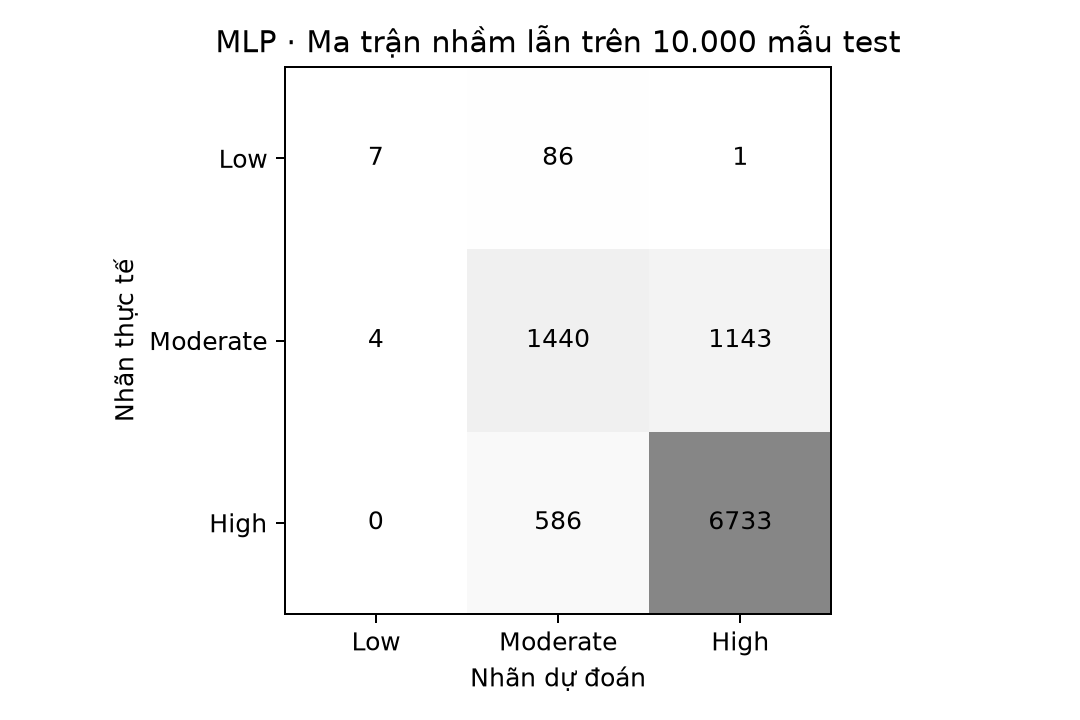
\includegraphics[width=.85\linewidth]{figures/confusion.png}\caption{Ma trận nhầm lẫn của MLP trên tập kiểm tra phân tầng.}\end{figure}
Tỷ lệ lỗi giữa Moderate và High cho thấy ranh giới của nhãn tổng hợp chưa được mô hình tách tốt. Cải thiện tiếp theo cần so sánh trọng số lớp, điều chỉnh ngưỡng và cách lấy mẫu trên validation, đồng thời giữ nguyên test để tránh chọn cấu hình theo kết quả test. Không đổi tên nhãn tổng hợp thành chẩn đoán y tế.
\section{Phân tích phần dư hồi quy}
\begin{figure}[htbp]\centering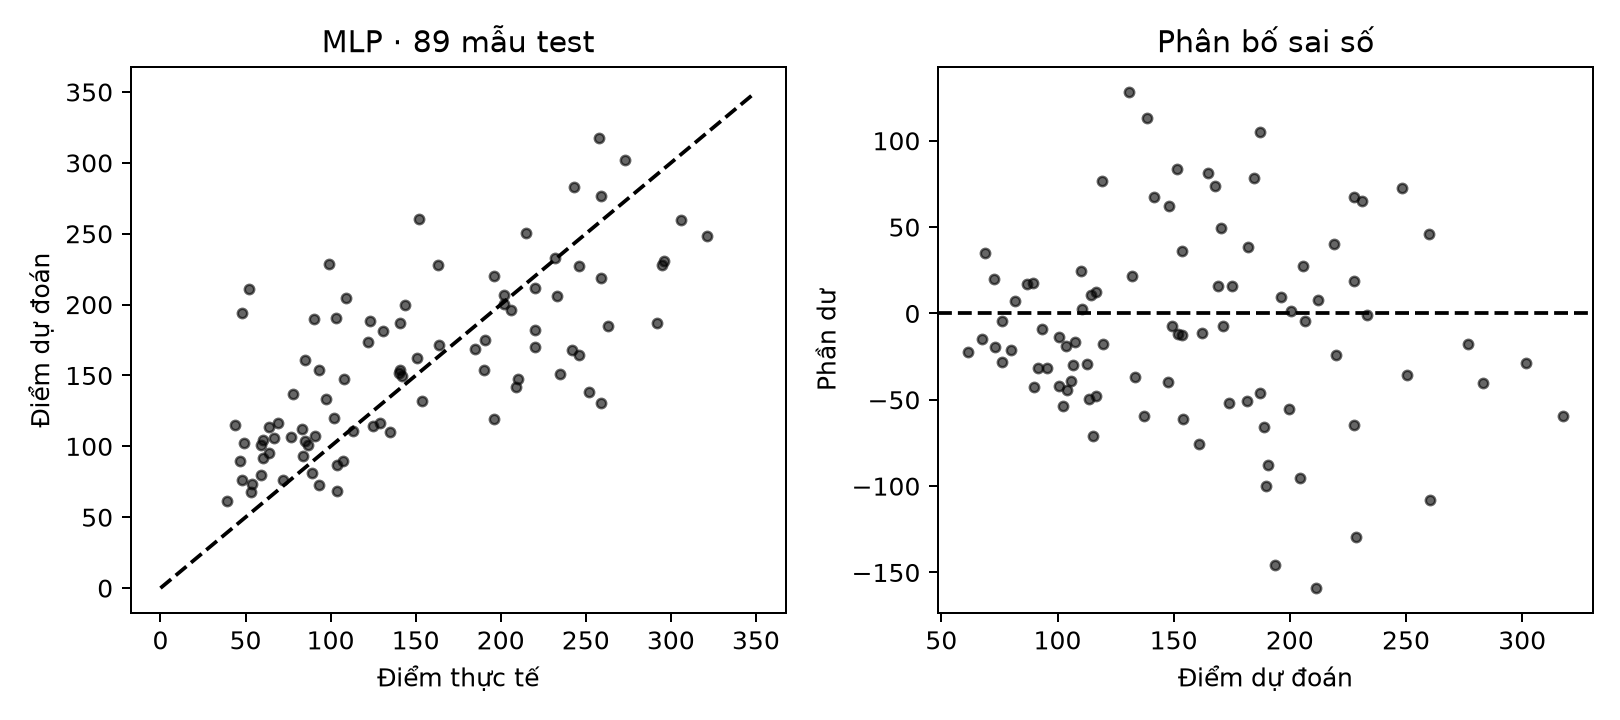
\includegraphics[width=\linewidth]{figures/regression.png}\caption{Dự đoán và phần dư của MLP trên 89 mẫu kiểm tra.}\end{figure}
Đường chéo thể hiện dự đoán bằng giá trị thật. Những điểm cách xa đường chéo đóng góp lớn vào MAE. Phần dư được tính bằng giá trị thực trừ dự đoán; phần dư dương biểu thị dự đoán thấp hơn thực tế. Không thể dùng một chỉ số tổng hợp để bảo đảm mọi nhóm đầu vào có sai số tương đương. Bản này chưa xây dựng khoảng dự báo và chưa hiệu chỉnh bất định.
\section{Hợp đồng dữ liệu và API}
GET /api/schema cung cấp thứ tự đặc trưng. GET /api/examples cung cấp một mẫu từ mỗi bộ dữ liệu để trình diễn. POST /api/chat nhận question, task và values. Với task knowledge, hệ thống truy xuất văn bản; với classification hoặc regression, values phải đủ các trường tương ứng. Kết quả gồm answer, result, sources, graph\_evidence và trace.

Trường result của phân loại gồm label, scores và scope. scores là đầu ra xác suất lớp của mô hình trên nhãn tổng hợp, chưa được hiệu chỉnh. Trường result của hồi quy gồm value và scope. Việc tách cấu trúc này tránh dùng chung một con số cho hai ý nghĩa khác nhau. Dữ liệu mẫu là mẫu của bộ nghiên cứu, không phải hồ sơ do người dùng cung cấp.

Nút ``Giải thích kết quả'' trên web gửi lại task và values của mẫu vừa chạy, nên câu trả lời được tính từ chính các đầu vào đó. Nhánh phân loại nêu nhãn, điểm của ba lớp, accuracy và macro-F1 trên tập test; nhánh hồi quy nêu điểm tiến triển, MAE và $R^2$. Mỗi nhánh đều giải thích ý nghĩa của nhãn/điểm và giới hạn khi chuyển sang trường hợp cá nhân. Mã tạo diễn giải nằm trong \path{app/model_explanation.py}; nó không sinh khuyến nghị điều trị.

Kiểm tra đầu vào hiện yêu cầu số hữu hạn, giới hạn trị tuyệt đối và đủ số trường. Đây là kiểm tra kỹ thuật, chưa phải kiểm định lâm sàng từng đơn vị. Giá trị nhập bằng số nhưng sai đơn vị vẫn có thể làm kết quả vô nghĩa; vì vậy demo được giới hạn ở dữ liệu nghiên cứu và có nút điền mẫu.
\section{Kết quả kiểm thử tích hợp}
Script test\_scenarios.py thực hiện tám trường hợp: câu hỏi có nguồn; câu hỏi ngoài từ vựng; suy luận phân loại; suy luận hồi quy; thiếu trường; giá trị không hữu hạn; tên bài toán không hợp lệ; lỗi Neo4j có kiểm soát. Tám trường hợp đều đạt điều kiện kiểm tra ở lần chạy lưu trong results/api\_scenarios.json. Kiểm tra lỗi cơ sở dữ liệu được thực hiện bằng thay thế driver trong test, không phải chủ động tắt cơ sở dữ liệu đang phục vụ người dùng.

Kiểm thử xác nhận hợp đồng phản hồi và nhánh lỗi, chưa đo độ chính xác truy xuất trên tập câu hỏi lớn. Trường hợp ngoài miền sử dụng chuỗi không có trong từ vựng, do đó không chứng minh hệ thống phát hiện mọi câu hỏi ngoài miền bằng tiếng Việt. Những giới hạn này giúp tách kiểm thử chức năng khỏi đánh giá chất lượng tư vấn.

Bản cập nhật thêm bảy điều kiện trong \path{scripts/test_chat_upgrade.py}: bốn chủ đề RAG mới, hai cách diễn giải kết quả mô hình và tổng số tài liệu công bố qua API. Thử nghiệm xác nhận các đoạn dẫn đúng nguồn và không biến điểm nghiên cứu thành chẩn đoán. Đây vẫn là kiểm tra chức năng theo kịch bản, chưa phải đánh giá y khoa bởi chuyên gia.
\section{Đối chiếu với sơ đồ yêu cầu}
\begin{longtable}{p{4cm}p{10cm}}\toprule Thành phần & Hiện thực trong sản phẩm\\\midrule
DB và Deep Learning & Hai bộ dữ liệu tách biệt, MLPClassifier và MLPRegressor; có checkpoint và kết quả test.\\
Phân loại và dự đoán & Hai lựa chọn trong phòng thực nghiệm, cùng chuyển kết quả đến phản hồi và nhật ký.\\
Web/sách đến KB & Kế thừa KB đã biên soạn từ tiểu luận 02; bảo toàn mã nguồn tài liệu, không tự động thu thập web ở thời điểm chạy.\\
KB và RAG & TF-IDF chọn đoạn văn; Neo4j trả các quan hệ cùng mã tài liệu; phản hồi trích đoạn có nguồn.\\
Agent và RL + rule & Handler và MessageBus xử lý yêu cầu; chính sách học một bước chọn kiểu phản hồi, luật chặn thiếu bằng chứng.\\
Tư vấn, trợ giúp & Chatbot giải thích kiến thức và phạm vi đầu ra; bản local dùng Qwen LoRA cho câu kiến thức có nguồn, còn câu thông số và thuốc theo luật.\\\bottomrule\end{longtable}

\chapter{KB, KG và RAG trong bộ sản phẩm nộp}
\section{Các thành phần có thể kiểm tra độc lập}
GlucoGuide lưu phần tri thức ở dạng dữ liệu và code, bên cạnh giao diện minh họa. Kho KB cung cấp nội dung và nguồn tham khảo; KG biểu diễn các quan hệ có hướng; RAG chọn căn cứ phù hợp cho từng câu hỏi. Ba phần dùng chung mã tài liệu để có thể truy từ một câu trả lời về đoạn văn và quan hệ đã sử dụng.

\begin{longtable}{p{2.2cm}p{6.6cm}p{5cm}}\caption{Các tệp chính trong bộ nộp tri thức.}\\\toprule Phần & Tệp & Nội dung\\\midrule\endfirsthead\toprule Phần & Tệp & Nội dung\\\midrule\endhead
KB & \path{kb/knowledge.json} & 46 đoạn, 19 nguồn, từ khóa, văn bản và bộ ba.\\
KG & \path{kg/nodes.csv}, \path{kg/relationships.csv} & 143 nút, 86 cạnh, mã tài liệu, trích đoạn và URL nguồn.\\
KG & \path{kg/graph.json}, \path{kg/import.cypher} & Bản chụp Neo4j đã đối chiếu và câu lệnh MERGE để nạp lại.\\
RAG & \path{rag/index.joblib}, \path{rag/settings.json} & Chỉ mục từ/ký tự đã fit và các ngưỡng đang sử dụng.\\
Đánh giá & \path{rag/queries.json}, \path{rag/evaluation.json} & Câu hỏi, tài liệu kỳ vọng, tài liệu được chọn và chỉ số tổng hợp.\\
Agent & \path{examples/agent_runs.json}, \path{code/} & Ví dụ chạy local, thông điệp giữa các agent và code truy vấn offline.\\
Toàn vẹn & \path{manifest.json} & Số lượng, kích thước và SHA-256 của từng tệp.\\\bottomrule\end{longtable}

Các tệp nằm trong \path{exports/diabetes/}; bản ZIP tương ứng là \path{exports/glucoguide_kb_kg_rag.zip}. Trọng số Qwen, mật khẩu Neo4j và trạng thái hội thoại cá nhân không được đưa vào gói. Phần code kèm theo đủ để truy vấn KB và bản chụp KG mà không cần mở web.
\productlink{Bộ tệp tri thức trên repository}{https://github.com/jellalaz/He_Thong_Thong_Minh_Thay_Que/tree/main/exports/diabetes}

\section{Agent đồ thị tham gia luồng trả lời}
\subsection{Trách nhiệm và hợp đồng thông điệp}
Agent Truy xuất nhận kế hoạch của lượt hỏi và trả tối đa bốn đoạn văn. Điều phối gửi danh sách mã tài liệu đó đến agent Đồ thị tri thức qua MessageBus. Handler của agent thực hiện truy vấn Neo4j và trả các trường: khái niệm đầu, quan hệ, khái niệm cuối, mã tài liệu, trích đoạn và URL nguồn. Nhật ký ghi REQUEST, INFORM hoặc FAILURE từ chính lần gọi handler.

Truy vấn sử dụng tham số \texttt{ids}; câu hỏi người dùng không được ghép vào mã Cypher. Bộ đọc lấy tối đa 48 quan hệ ứng viên và chọn tối đa 12 quan hệ cho ngữ cảnh. Khi nhiều tài liệu cùng có căn cứ, các quan hệ được lấy luân phiên theo tài liệu để một đoạn không chiếm toàn bộ phần đồ thị.

\begin{Verbatim}[fontsize=\small,breaklines=true]
MATCH (a:Concept)-[r:RELATED_TO]->(b:Concept)
WHERE r.document IN $ids
RETURN a.name AS source, r.label AS relation,
       b.name AS target, r.document AS document,
       r.evidence AS evidence, r.source_url AS source_url
ORDER BY document, source, relation, target LIMIT 48
\end{Verbatim}

\subsection{Đối chiếu căn cứ trước khi đưa vào mô hình}
Một cạnh chỉ được chấp nhận khi mã tài liệu thuộc nhóm đã truy xuất, bộ ba khớp dữ liệu KB, trích đoạn khớp văn bản và URL khớp nguồn của đoạn đó. Quan hệ trùng bị bỏ. Cạnh không khớp không được đưa vào prompt, kể cả khi nó tồn tại trong cơ sở dữ liệu.

Những cạnh đã đạt kiểm tra được trình bày cùng văn bản dưới dạng ``khái niệm đầu $\rightarrow$ quan hệ $\rightarrow$ khái niệm cuối'', kèm mã tài liệu. Qwen nhận cả hai dạng căn cứ trong cùng yêu cầu local. Bước kiểm chứng phản hồi tiếp tục đối chiếu mã nguồn, số liệu và phạm vi; nó không phải một cơ chế chứng minh mọi suy luận của mô hình đều đúng.

Trường \texttt{graph\_context\_supplied} cho biết phản hồi Qwen được chấp nhận có ngữ cảnh đồ thị hay không. Trường này ghi nhận dữ liệu đã cấp vào đường sinh, không đo mức độ mô hình thực sự dựa vào từng cạnh. Các cạnh hiển thị cùng phản hồi được giới hạn theo những tài liệu mà bản sinh đã dẫn mã.

\subsection{Mất kết nối và thứ tự ưu tiên}
Khi Neo4j không hoạt động, MessageBus ghi FAILURE của agent đồ thị. Hệ thống tiếp tục bằng văn bản KB, để trạng thái đồ thị là unavailable và không tạo các quan hệ thay thế. Bản truy vấn offline dùng dữ liệu đã xuất chỉ khi người chạy chủ động chọn công cụ đi kèm; đầu ra ghi rõ exported-snapshot.

Nhánh cấp cứu được phân loại trước toàn bộ bước truy xuất. Nó không chờ KG, chỉ mục RAG hoặc Qwen. Do đó việc bổ sung đồ thị không thay đổi thứ tự xử lý các tình huống cần hành động ưu tiên.

\section{Xuất và chạy lại bộ nộp}
\subsection{Kiểm tra nguồn trước khi xuất}
Script \path{scripts/export_knowledge.py} chỉ kết nối Neo4j trên loopback. Nó đọc toàn bộ nút và cạnh Concept, đối chiếu chính xác tập bộ ba với KB, rồi kiểm tra trích đoạn và URL. Nếu hai nguồn không khớp, thao tác xuất dừng thay vì ghi một bản chụp thiếu hoặc tự dựng dữ liệu từ hình ảnh.

CSV dùng UTF-8 có BOM để giữ chữ tiếng Việt khi mở bằng các công cụ bảng tính trên Windows. Định danh n0001, n0002 và các giá trị tiếp theo là mã của bộ xuất, không phải ID nội bộ Neo4j. JSON bảo toàn tên khái niệm, quan hệ, tài liệu và bằng chứng; Cypher dùng MERGE nên có thể nạp các dữ liệu tương ứng mà không cần xóa cơ sở dữ liệu đang có.

\subsection{Chỉ mục và cấu hình RAG}
Chỉ mục đã fit chứa hai bộ vector hóa, ma trận tài liệu và danh mục đoạn văn. Cấu hình đi kèm ghi n-gram từ 1--2, n-gram ký tự 3--5, trọng số 0,55/0,45, ngưỡng điểm 0,15, tỷ lệ so với đoạn đầu 0,58 và tối đa bốn kết quả. Code của bộ truy xuất được lưu cùng gói để đọc lại đối tượng joblib.

Checksum được kiểm tra trước khi nạp chỉ mục. Joblib vẫn là định dạng chỉ nên mở từ nguồn tin cậy; SHA-256 giúp phát hiện tệp bị thay đổi, không xác thực danh tính người phát hành. Phiên bản thư viện được ghi trong requirements của bộ nộp để làm rõ điều kiện tái lập.

\subsection{Lệnh sử dụng}
Từ project gốc, xuất dữ liệu và lấy các ví dụ hội thoại trên máy:
\begin{Verbatim}[fontsize=\small,breaklines=true]
python -m scripts.export_knowledge --live-examples
python -m scripts.test_knowledge_export
\end{Verbatim}
Từ thư mục \path{exports/diabetes/}, truy vấn bộ nộp không cần web hoặc kết nối mạng:
\begin{Verbatim}[fontsize=\small,breaklines=true]
python code/scripts/query_knowledge_export.py . --question "HbA1c là gì?"
\end{Verbatim}
Lệnh này chạy các agent truy xuất, đồ thị bản chụp và tổng hợp căn cứ. Nó không chạy Qwen hoặc giả lập một phản hồi ngôn ngữ sinh. Muốn trình diễn hội thoại đầy đủ, dùng ứng dụng local trong project gốc. Để nạp lại vào Neo4j local, dùng \path{code/scripts/restore_knowledge_export.py}; thông tin đăng nhập được nhập riêng, không lưu trong gói.

\section{Kết quả kiểm tra}
\begin{longtable}{p{8.5cm}p{5.3cm}}\caption{Kết quả truy xuất và kiểm tra bộ nộp.}\\\toprule Hạng mục & Kết quả\\\midrule
Số tệp trong bộ nộp & 26\\
Câu hỏi truy xuất & 22\\
Hit@1 & 90.0\%\\
Hit@4 & 100.0\%\\
MRR@4 & 0.950\\
Kiểm tra agent đạt & 11\\
Kiểm tra bộ nộp đạt & 8\\\bottomrule\end{longtable}
Tập truy xuất gồm 20 câu có tài liệu kỳ vọng và hai câu cần không trả tài liệu. Câu hỏi bao phủ kiến thức bệnh, bữa ăn, thuốc ở mức thông tin, vận động, theo dõi, câu không dấu và một lượt hỏi tiếp. Danh sách tài liệu kỳ vọng được ghi trước khi chạy phép đo. Đây là tập kiểm tra chức năng do project biên soạn, chưa phải một benchmark y khoa độc lập.

Hit@1 đo tỷ lệ câu có tài liệu kỳ vọng ở vị trí đầu. Hit@4 đo tỷ lệ tìm thấy ít nhất một tài liệu kỳ vọng trong danh sách trả về; danh sách có thể ngắn hơn bốn đoạn. MRR@4 là trung bình nghịch đảo thứ hạng đúng đầu tiên. Các chỉ số này đánh giá bước truy xuất, không phải độ chính xác chẩn đoán hay mức an toàn của toàn bộ câu trả lời.

Bộ kiểm tra gói nộp phát lại 22 truy vấn từ chỉ mục đã lưu khi socket bị vô hiệu hóa; đối chiếu CSV, JSON và ZIP; chạy entry point bằng các module đã đóng gói; phát hiện tệp bị sửa; và dùng EXPLAIN để kiểm tra Cypher mà không thực hiện ghi dữ liệu. Các kiểm tra agent riêng xét nguồn sai, bộ ba sai, mã tài liệu lạ, bản ghi trùng, việc cấp KG vào prompt, mất Neo4j và nhánh cấp cứu.

Ba ví dụ thông thường chạy trên Qwen local đều trả phản hồi được chấp nhận với hai quan hệ có nguồn. Ví dụ đường huyết cao kèm nôn, đau bụng đi theo luật cấp cứu và không gọi bước sinh. Các phản hồi và trace nguyên văn nằm trong \path{examples/agent_runs.json}; số ví dụ nhỏ này chỉ dùng để đối chiếu luồng thực thi.

\section{Phạm vi và giới hạn}
KG hiện còn 57 cụm rời nhau và nhiều cụm chỉ có hai hoặc ba khái niệm. Hệ thống truy vấn quan hệ theo tài liệu đã chọn, chưa tìm đường nhiều bước, chưa hợp nhất một ontology y khoa và chưa triển khai thuật toán cộng đồng của Microsoft GraphRAG. Mở rộng các bước đó cần thêm bài toán đánh giá cụ thể, không thể chỉ dựa vào việc đồ thị có nhiều nút hơn.

Các agent cùng chạy trong một tiến trình dưới điều phối tập trung. Cách tổ chức cho phép quan sát giao thức và kiểm thử từng vai trò, nhưng chưa chứng minh lợi ích của các agent tự chủ độc lập. Chất lượng nội dung vẫn phụ thuộc nguồn, độ phủ KB, cách biên soạn bộ ba và kiểm tra đầu ra. Trước khi áp dụng ngoài thực nghiệm học phần cần có đánh giá chuyên môn và dữ liệu phù hợp.

\chapter{Code và demo}
\section{Địa chỉ và cách chạy}
\noindent\textbf{Bản hoàn thiện chạy trên máy cá nhân}\par
\noindent\url{http://localhost:8765}\par\medskip
\noindent\textbf{Xem đồ thị trên web, không cần nhập lệnh}\par
\noindent\url{http://localhost:8765/\#graph}\par\medskip
\noindent\textbf{Neo4j Browser cục bộ}\par
\noindent\url{http://localhost:7474/browser/}\par\medskip
\noindent\textbf{Kho mã nguồn}\par
\noindent\url{https://github.com/jellalaz/He_Thong_Thong_Minh_Thay_Que}\par\medskip
\noindent\textbf{Demo Vercel của phiên bản trước}\par
\noindent\url{https://glucoguide-giang254.vercel.app}\par\medskip
Các địa chỉ localhost chỉ truy cập dịch vụ trên máy đang chạy sản phẩm. Bản hoàn thiện dùng Qwen3 4B và Neo4j local; không thể mở từ máy khác bằng các địa chỉ này. Bản Vercel là triển khai trước đây, chưa được xác nhận đồng bộ mô hình, đồ thị và luật an toàn mới.


Trên máy thực nghiệm, chạy \path{start-neo4j.ps1} nếu cơ sở dữ liệu chưa hoạt động, rồi mở \path{START_CHATBOT_LOCAL.cmd} để khởi động Qwen và web. Tệp requirements.txt mô tả thư viện ứng dụng; requirements-training.txt dành cho tái lập huấn luyện. Các script \path{scripts/train_models.py}, \path{scripts/train_policy.py} và \path{scripts/ingest_graph.py} lần lượt tạo checkpoint, chính sách và dữ liệu đồ thị. Quá trình phục vụ dùng tài nguyên đã có trên máy, không tự tải mô hình hoặc tài liệu. Cấu hình Neo4j nằm trong .env và không đưa lên repository.
\section{Kịch bản trình diễn}
Kịch bản thứ nhất: hỏi ``HbA1c là gì?''. Kiểm tra nội dung, mở nguồn tham khảo, đối chiếu bước truy xuất và số quan hệ Neo4j. Kịch bản thứ hai: hỏi một chủ đề không có trong kho, chẳng hạn lịch sử một đội bóng. Hệ thống phải nêu phạm vi hỗ trợ hoặc hỏi làm rõ, không tự tạo nguồn.

Kịch bản thứ ba: nhập đủ tám trường phân loại bằng một mẫu của dữ liệu. Ghi lại nhãn, thông báo phạm vi và nhật ký mô hình. Kịch bản thứ tư: nhập đủ mười trường hồi quy từ mẫu nghiên cứu, kiểm tra đầu ra số và thông báo đây là điểm tiến triển. Hai kịch bản không dùng chung biểu mẫu.

Kịch bản thứ năm: bỏ một trường bắt buộc. Hệ thống phải nêu trường còn thiếu. Kịch bản thứ sáu: nhập giá trị không hữu hạn hoặc chuỗi ký tự vào API, hệ thống phải từ chối. Kịch bản thứ bảy: dùng kiểm thử giả lập Neo4j mất kết nối để kiểm tra nhánh dự phòng; không cần tắt dịch vụ đang phục vụ người dùng. Kịch bản thứ tám: mở Neo4j Browser và thực hiện truy vấn dưới đây để đối chiếu với giao diện đồ thị.
\begin{verbatim}
MATCH (a:Concept)-[r:RELATED_TO]->(b:Concept)
RETURN a,r,b LIMIT 100;
\end{verbatim}
\section{Hạn chế và hướng hoàn thiện}
Hệ thống duy trì ngữ cảnh chủ đề trong phiên nhưng chưa có bộ nhớ hội thoại bền vững, chưa đọc phiếu xét nghiệm, nhánh Qwen local mới được đánh giá trên tập nội bộ nhỏ và chưa có hội đồng tranh biện độc lập. Kiểm chứng mô hình mới chỉ dùng một seed; chưa có đánh giá chuyên gia, chưa có dữ liệu ngoài miền và chưa kiểm thử tải lớn. RL học quy trình mô phỏng, không quyết định điều trị.

Hướng ưu tiên là mở rộng tập câu hỏi độc lập, kiểm tra đơn vị có nguồn và đánh giá vai trò của KG bằng phép loại bỏ thành phần trên cùng tập câu hỏi. Chất lượng nguồn và khả năng phát hiện thiếu căn cứ cần được đo cùng độ đúng chủ đề và thời gian trả lời.

\section{Triển khai công khai trên Vercel và Neo4j Aura}
\productlink{GlucoGuide -- bản demo công khai}{https://glucoguide-giang254.vercel.app}
\subsection{Kiến trúc triển khai}
Vercel Hobby phục vụ giao diện và API FastAPI từ cùng tên miền. Các checkpoint được đóng gói cùng mã nguồn; đồ thị nằm trên Neo4j AuraDB Free. Vì vậy bản demo không phụ thuộc tiến trình chạy trên máy cá nhân. Người xem không cần cài Neo4j hoặc đăng nhập để sử dụng bốn chức năng trên web.

Các biến môi trường kết nối (URI, tài khoản, mật khẩu và tên cơ sở dữ liệu) được cấu hình trên máy chủ. Trình duyệt gọi API của ứng dụng, không nhận thông tin đăng nhập cơ sở dữ liệu. Các tệp môi trường, dữ liệu thô và tài liệu báo cáo không được đóng gói vào hàm phục vụ web.
\subsection{Nạp dữ liệu và kiểm tra}
Script \path{scripts/ingest_graph.py} nạp kho tri thức theo phép MERGE để có thể chạy lại. Tùy chọn \texttt{--https} sử dụng Query API khi môi trường phát triển không kết nối được Bolt. Đồ thị triển khai có 60 nút Concept và 32 quan hệ; kho văn bản gồm 21 đoạn kiến thức.

Ngày 05/11/2026, script \path{scripts/check_deployment.py} đã kiểm tra thành công 12 nhóm điều kiện trên địa chỉ công khai, gồm tải giao diện, trạng thái cơ sở dữ liệu, đồ thị, hội thoại có căn cứ, câu hỏi tiếp nối, thiếu đơn vị, câu ngoài phạm vi, nhận diện tình huống cần trợ giúp, hai bài toán mô hình, dữ liệu đầu vào không hợp lệ và tra cứu KB. Kết quả lưu tại \path{results/deployment_checks.json}. Kiểm tra này xác nhận các tình huống đã chạy; không thay thế đánh giá chuyên gia hoặc kiểm thử tải.
\subsection{Vận hành trong gói miễn phí}
Triển khai sử dụng Vercel Hobby và AuraDB Free. Không bật dịch vụ trả phí. Tài nguyên và thời gian đáp ứng phụ thuộc giới hạn của hai gói; lần gọi đầu có thể chậm do khởi động hàm. Chủ tài khoản cần theo dõi trạng thái Aura khi lâu không sử dụng, giữ bản sao dữ liệu và có thể nạp lại bằng script đã cung cấp.

Để xem trực tiếp bằng Neo4j, chủ tài khoản mở Aura Console, chọn instance và mục Query; thực hiện câu lệnh MATCH trong kịch bản trình diễn. Khách xem dùng mục Đồ thị trên web. Bản Neo4j cục bộ vẫn dùng được cho phát triển nhưng không phải điều kiện để demo công khai hoạt động.

\chapter{Tinh chỉnh mô hình hội thoại trên máy cá nhân}
\section{Mục tiêu và phạm vi}
Các câu hỏi thử cho thấy phản hồi theo mẫu còn cứng và dễ thiếu bối cảnh. Nhánh hội thoại cục bộ bổ sung Qwen3 1.7B để diễn đạt kiến thức lấy từ KB. Mô hình nền đã được Qwen tiền huấn luyện; thực nghiệm này chỉ tinh chỉnh LoRA trên ví dụ tiếng Việt của project. Việc tải mô hình không được tính là một lần huấn luyện.

Suy luận diễn ra trên máy cá nhân, không gọi dịch vụ mô hình ngôn ngữ bên ngoài. Bản Vercel tiếp tục phục vụ KB, luật và các mô hình dữ liệu bảng; checkpoint Qwen không chạy trong hàm Vercel. Hai chế độ dùng chung giao diện nhưng có điều kiện vận hành khác nhau.
\section{Dữ liệu và thiết kế đánh giá}
\subsection{Nguồn và cách xây dựng}
Tệp \path{experiments/local_qwen/dataset.json} chứa các cặp chỉ dẫn và phản hồi do project biên soạn từ các đoạn KB có nguồn. Mỗi mẫu lưu câu hỏi, lịch sử, mã đoạn kiến thức và câu trả lời đích. Nguồn KB gồm các tài liệu sức khỏe đã liệt kê trong danh mục. Đây không phải dữ liệu bệnh án và chưa được chuyên gia y tế thẩm định.

Tập huấn luyện gồm 76 mẫu; tập validation gồm 21 mẫu diễn đạt khác nhưng cùng nguồn KB. Tập test gồm 16 mẫu, chia đều thành nhóm kiến thức và nhóm hội thoại. Kiểm tra chuẩn hóa câu hỏi loại trùng lặp trực tiếp giữa các tập. Tuy vậy, cùng nguồn và cùng cách biên soạn làm giới hạn tính độc lập của đánh giá. Hai nhóm test không được gọi là hai bộ dữ liệu lâm sàng độc lập.
\subsection{Đối chiếu trước và sau tinh chỉnh}
Mô hình nền và checkpoint LoRA nhận cùng tài liệu, câu hỏi, lịch sử và giới hạn sinh. Chọn checkpoint bằng loss validation, không dùng điểm test để chọn epoch. Nhóm kiến thức kiểm tra trả lời đúng trọng tâm và dẫn mã nguồn; nhóm hội thoại kiểm tra thông tin thiếu, câu hỏi tiếp nối, lời cảm ơn, yêu cầu thuốc và câu ngoài phạm vi. Loss giảm chỉ cho thấy mô hình khớp câu trả lời đích tốt hơn; không đủ kết luận độ chính xác y tế tăng.
\section{Cấu hình và quá trình học}
Máy thực nghiệm có Intel Core i9-14900HX, RAM khoảng 16 GB và NVIDIA GeForce RTX 4060 Laptop GPU 8 GB. Mô hình nền được tải từ kho chính thức:
\productlink{Qwen3 1.7B}{https://huggingface.co/Qwen/Qwen3-1.7B}

LoRA giữ cố định trọng số nền $W$ và học hai ma trận nhỏ để tạo $W'=W+\frac{\alpha}{r}BA$. Cấu hình dùng hạng $r=8$, $\alpha=16$, dropout 0,05, áp dụng vào các phép chiếu query và value. Hàm mất mát chỉ tính trên token câu trả lời, bỏ qua phần chỉ dẫn và tài liệu.

Batch size bằng 1 nghĩa là một mẫu được xử lý trong mỗi lượt lan truyền; tích lũy gradient qua 4 mẫu trước khi cập nhật. Một epoch đi qua toàn bộ tập train. AdamW cập nhật tham số từ gradient với learning rate $10^{-4}$. Thực nghiệm đặt 3 epoch, tối đa 768 token cho một mẫu, dùng BF16 và gradient checkpointing để giảm bộ nhớ. Training loss theo bước và validation loss theo epoch được lưu riêng để theo dõi khả năng khái quát hóa.
\subsection{Kết quả đo trên máy thực nghiệm}
Số tham số được tối ưu là 1,605,632, trên tổng 1,722,180,608 tham số. Checkpoint được chọn ở epoch 3. Loss validation của mô hình nền là 1.0810; giá trị tốt nhất sau tinh chỉnh là 0.0082. Thời gian ba epoch, gồm đánh giá validation và lưu checkpoint, là 1.97 phút. Bộ nhớ GPU cấp phát đỉnh do PyTorch ghi nhận là 3.93 GiB; số này không bao gồm toàn bộ bộ nhớ các ứng dụng khác.
\begin{figure}[htbp]\centering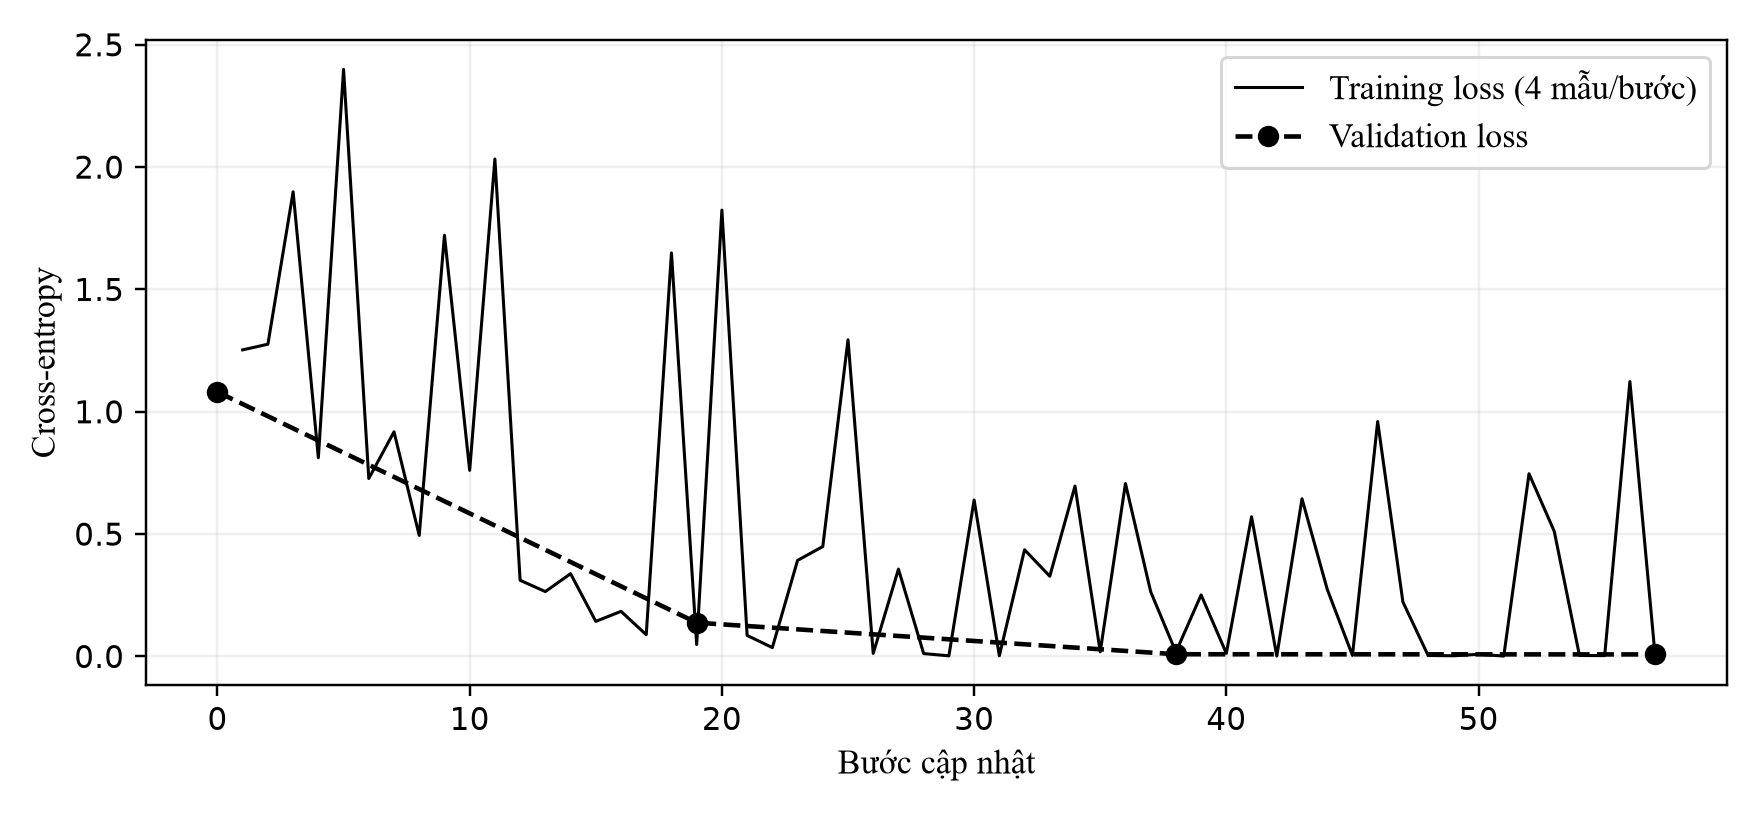
\includegraphics[width=\linewidth]{figures/qwen_learning.png}\caption{Loss huấn luyện theo bước và validation theo epoch. Điểm đầu validation thuộc mô hình nền.}\end{figure}
\begin{table}[H]\centering\small
\begin{tabular}{llrrrr}\toprule
Mô hình & Nhóm & Có dẫn mã & Mã lạ & Chạm giới hạn & Giây/câu\\\midrule
Qwen nền & Kiến thức & 0/8 & 0 & 0 & 8.07\\
Qwen nền & Hội thoại & 0/8 & 0 & 0 & 4.97\\
Qwen LoRA & Kiến thức & 8/8 & 0 & 0 & 7.57\\
Qwen LoRA & Hội thoại & 7/8 & 1 & 0 & 4.93\\
\bottomrule\end{tabular}
\caption{Kiểm tra hình thức đầu ra trên hai nhóm test, mỗi nhóm 8 câu.}\end{table}
Có dẫn mã chỉ kiểm tra sự xuất hiện của mã tài liệu, không chứng minh trích dẫn hỗ trợ đầy đủ câu trả lời. Mã lạ là mã không nằm trong ngữ cảnh đã cấp. Chạm giới hạn nghĩa là sinh đủ 320 token, có nguy cơ câu bị cắt. Độ trễ được đo sau khi mô hình đã nạp, không gồm thời gian khởi động hoặc truy xuất Neo4j. Hai mô hình dùng cùng ngữ cảnh được chỉ định trước để tách ảnh hưởng của bộ sinh; kết quả này chưa đo toàn bộ pipeline truy xuất.

Tệp \path{results/local_qwen/base_answers.json} và \path{results/local_qwen/lora_answers.json} lưu nguyên văn từng phản hồi. Tệp \path{results/local_qwen/training_summary.json} lưu cấu hình, mã băm dữ liệu và tài nguyên đo được. Các tệp này cho phép kiểm tra lại kết luận mà không cần dựa vào ảnh minh họa.

\subsection{Phân tích phản hồi và giới hạn}
Trên nhóm kiến thức, checkpoint LoRA bám sát các đoạn KB hơn: câu hỏi chia bữa ăn không còn tự thêm số gram; câu hỏi về carbohydrate không còn suy diễn nguyên nhân bệnh ngoài tài liệu. Tuy nhiên, phần lớn phản hồi gần với văn bản KB. Kết quả chủ yếu cho thấy khả năng tuân thủ ngữ cảnh và định dạng, chưa chứng minh suy luận y khoa mới.

Ở nhóm hội thoại, mô hình thuần vẫn có hạn chế: lời bày tỏ thân thiện bị trả lời cứng và kèm mã nguồn không tồn tại; câu thiếu đơn vị HbA1c và câu hỏi tiếp nối chưa được làm rõ đầy đủ. Do đó bản ứng dụng không dùng trực tiếp đầu ra Qwen cho các trường hợp này, mà giữ định tuyến hội thoại và luật kiểm tra thông số. Loss validation rất thấp cần được đọc cùng thực tế rằng train và validation dùng chung đoạn nguồn và nhiều câu trả lời đích. Một nghiên cứu tiếp theo cần tập nguồn độc lập, cách diễn đạt đa dạng hơn và đánh giá chuyên gia.
\subsection{Lượt tinh chỉnh hội thoại thứ hai}
Sau khi phát hiện các câu ``bạn là ai'' và ``Giới thiệu đi'' bị ghép tài liệu không liên quan, nhóm biên soạn thêm 20 mẫu train và 6 mẫu validation về giới thiệu, lời phàn nàn và thay đổi chủ đề; giữ 8 câu xã giao làm test, trong đó có câu do người dùng thử. Lượt train này trộn 26 mẫu kiến thức cũ để hạn chế quên nhiệm vụ trước, tổng cộng 46 train, 13 validation và 16 test. Qwen LoRA khởi đầu từ adapter lượt một, tiếp tục 3 epoch với learning rate $3\cdot10^{-5}$ trên cùng GPU. Validation loss giảm từ 0,5873 xuống 0,5201 trong khoảng 70 giây.

Đọc nguyên văn tám câu test xã giao cho thấy cải thiện chưa đủ tin cậy: một số câu tốt hơn nhưng vẫn có câu lặp chỉ dẫn hệ thống hoặc đáp sai sắc thái lời phàn nàn. Do đó checkpoint của lượt hai được giữ trong \path{.local-training/qwen-round2} để nghiên cứu, không đóng gói vào sản phẩm. Mô hình đang dùng vẫn là adapter kiến thức lượt một. Các lượt giới thiệu, chào hỏi và góp ý được định tuyến riêng, không truy xuất nguồn y tế chỉ vì trong lịch sử có câu về bệnh. Kiểm thử thực tế gồm 37 tình huống chatbot.

\subsection{Phản hồi hữu ích và chính sách Q cục bộ}
Project đã có bảng Q huấn luyện trên môi trường mô phỏng để quyết định khi nào hỏi làm rõ, dẫn nguồn hoặc giải thích mô hình. Bản local nay bổ sung nút ``Hữu ích'' và ``Chưa hữu ích'' dưới câu trả lời kiến thức. Phản hồi $r\in\{+1,-1\}$ cập nhật bảng Q một bước cho hai cách trình bày: trực tiếp hoặc hỏi nhu cầu hướng dẫn từng bước, theo $Q\leftarrow Q+0,2(r-Q)$. Bảng được lưu trên máy trong \path{.local-training/feedback_q.json}; không lưu nội dung hội thoại trong tệp này.

Chính sách mới chỉ điều chỉnh cách trình bày, không đổi ngưỡng y tế, liều thuốc, nhánh khẩn cấp hay mô hình phân loại. Phản hồi không tự cập nhật trọng số Qwen. Khi chưa có đủ đánh giá, đây là thích nghi đơn giản theo từng lượt, chưa chứng minh câu trả lời y khoa chính xác hơn. Nút phản hồi chỉ hiện ở demo local có tiến trình lưu trạng thái; bản Vercel vẫn dùng chính sách mô phỏng đã đóng gói.
\section{Phối hợp đa agent khi trả lời}
\begin{figure}[htbp]\centering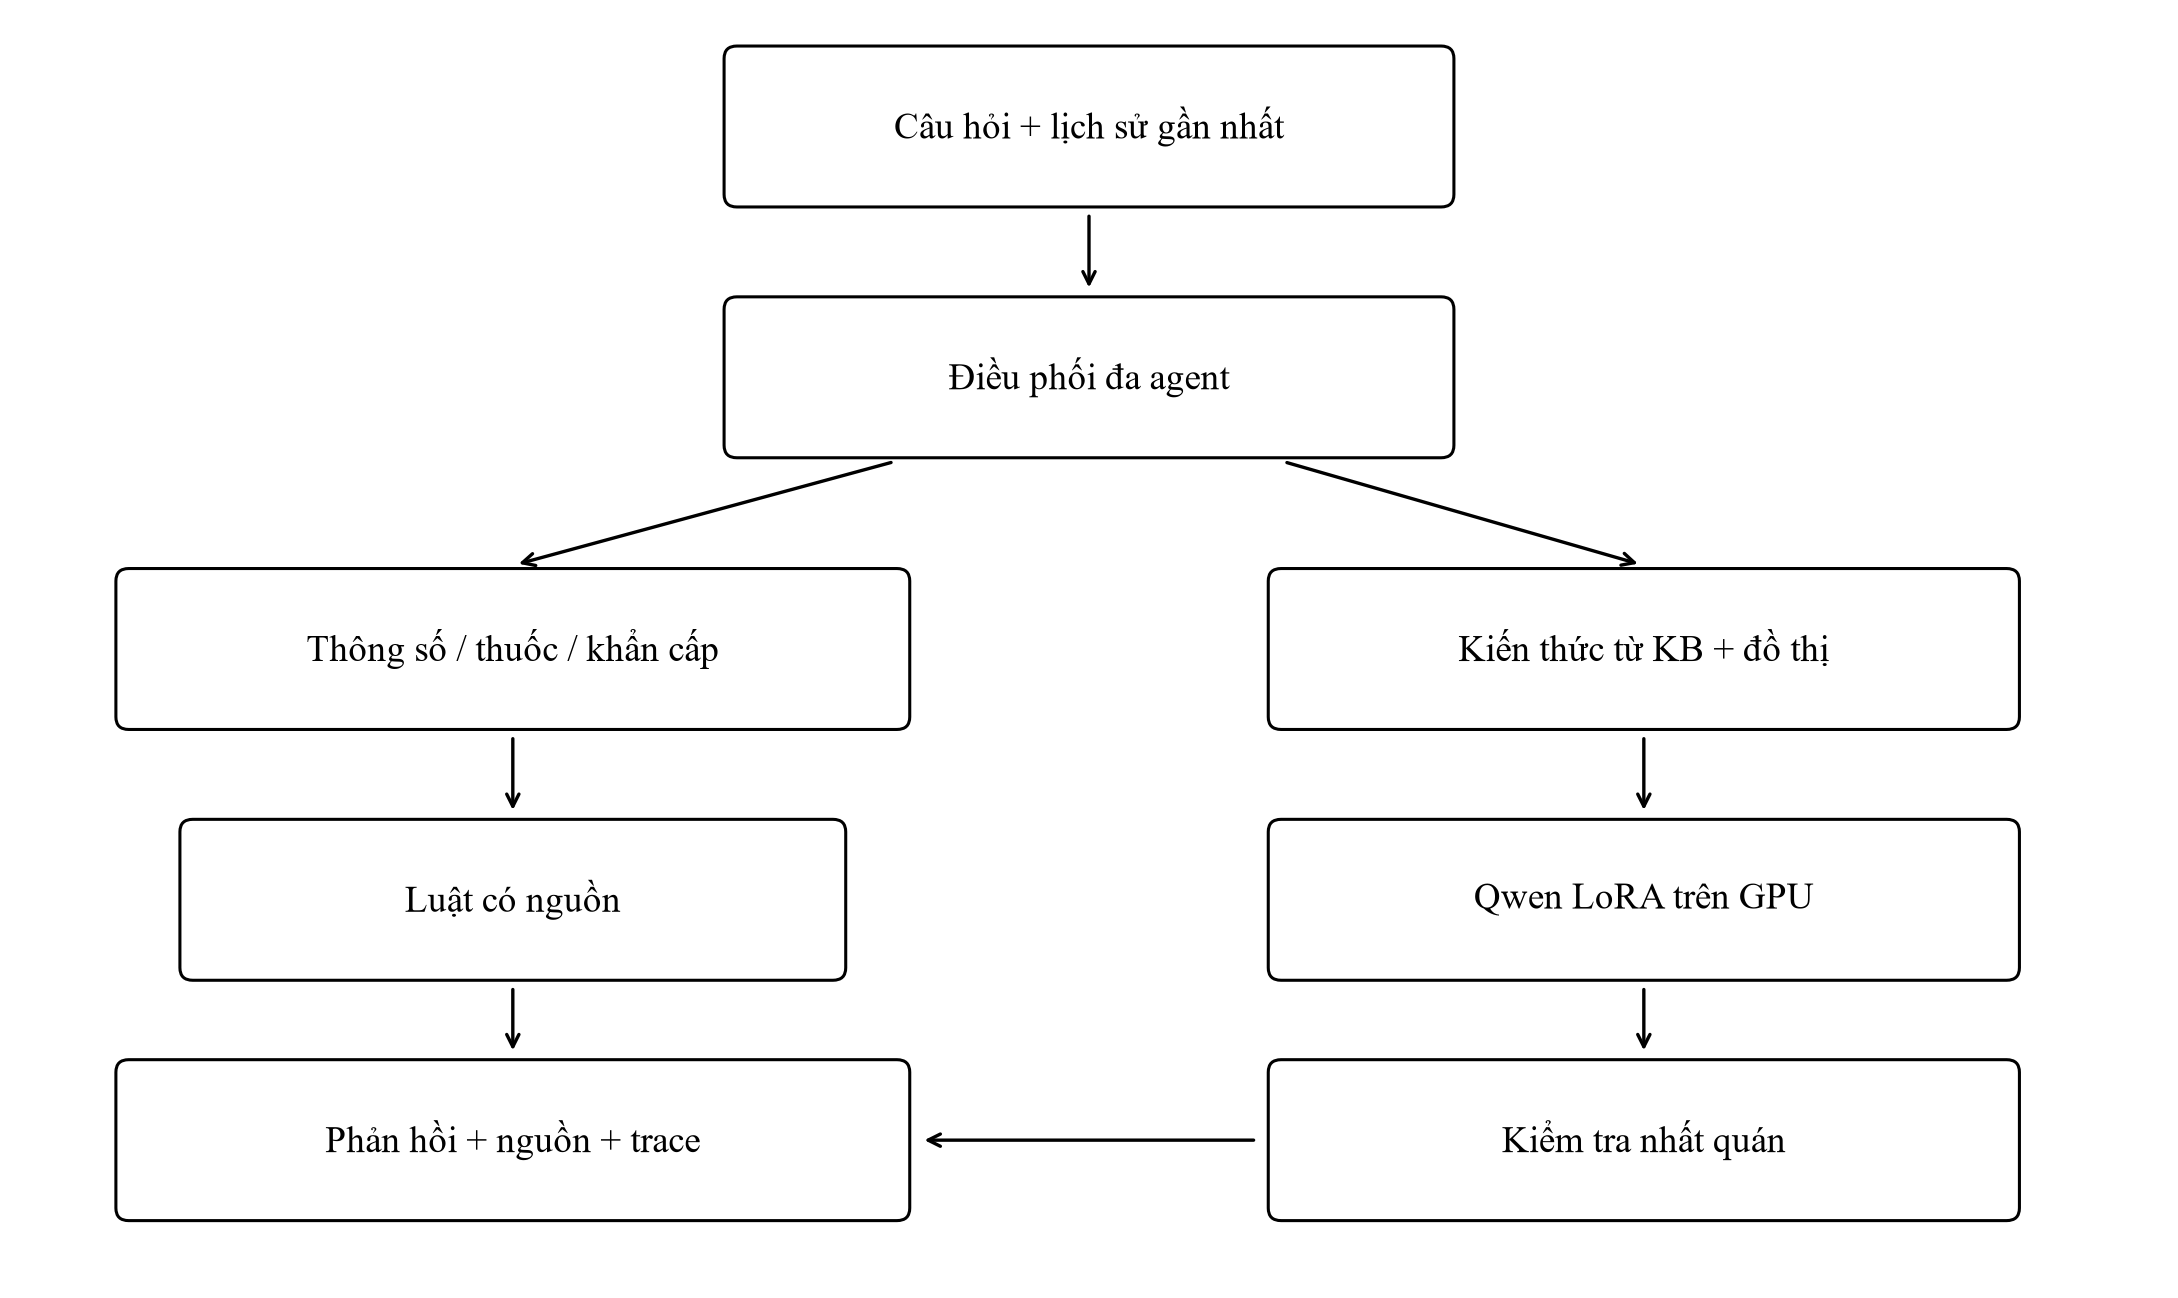
\includegraphics[width=\linewidth]{figures/local_architecture.png}\caption{Luồng xử lý tại máy cá nhân; phản hồi không đạt kiểm tra quay về nội dung KB.}\end{figure}
Điều phối xác định loại yêu cầu, truy xuất đoạn KB và gửi thông điệp đến agent ngôn ngữ cục bộ khi phù hợp. Agent kiểm chứng đối chiếu mã trích dẫn, số liệu và một số biểu thức không được phép trước khi chuyển câu trả lời ra giao diện. Nếu tải mô hình thất bại hoặc bản sinh không đạt kiểm tra, hệ thống trả về nội dung KB và ghi nguyên nhân trong trace.

Câu chứa thông số, câu về thuốc và tình huống khẩn cấp được ưu tiên xử lý bằng luật có nguồn. Qwen không được tự quyết định liều thuốc hay xác nhận bệnh. Bộ kiểm chứng hiện tại là bộ lọc nhất quán, chưa kiểm tra được mọi sai lệch ngữ nghĩa. Lịch sử gần nhất hỗ trợ diễn đạt nối tiếp; lịch sử gửi từ trình duyệt không phải bộ nhớ bền vững giữa các phiên.
\subsection{Huấn luyện lại bộ nhận diện ý định}
Bên cạnh LoRA, project huấn luyện một bộ định tuyến câu hỏi tiếng Việt bằng TF--IDF ký tự và hồi quy logistic. Bộ ví dụ gốc có 64 câu train và 16 câu test; sau khi bổ sung các cách hỏi về ăn uống, trái cây, vận động, thuốc, theo dõi, huyết áp, HbA1c và câu ngoài phạm vi, tập có 112 câu train và 32 câu test. Các câu test không được đưa vào bước fit. Trên tập test nội bộ này, accuracy đạt 93,75\% và macro-F1 đạt 0,937. Mã, dữ liệu, checkpoint và dự đoán từng câu nằm tại \path{scripts/train_intent.py}, \path{data/intent_expansion.json}, \path{models/chat_intent.joblib} và \path{results/intent_evaluation.json}.

Tập ví dụ do project tự viết, cùng chủ đề và một số từ khóa xuất hiện ở cả hai tập; đây là phép thử định tuyến hẹp, không phải đánh giá hội thoại ngoài miền. Bộ này không cập nhật trọng số Qwen và không cải thiện độ chính xác của hai mô hình dữ liệu bảng. Các tình huống xã giao, thông số, thuốc và khẩn cấp vẫn có luật ưu tiên.
\section{Tái lập và vận hành}
Chạy \path{experiments/local_qwen/train.py} bằng môi trường \path{.venv-llm} để tạo checkpoint, log loss và phản hồi kiểm thử. Adapter dùng để chạy được đóng gói tại \path{models/qwen_adapter}; checkpoint huấn luyện gốc nằm tại \path{.local-training/qwen-lora/best}. Mô hình nền và cache được lưu ngoài Git vì dung lượng lớn. Sau khi có đủ tệp, chế độ suy luận đặt biến offline để không tải tài nguyên từ mạng.

Khởi động bằng \path{run-local-qwen.ps1}, giữ cửa sổ tiến trình hoạt động và mở:
\productlink{Demo Qwen cục bộ}{http://localhost:8766}
Địa chỉ này chỉ dùng trên máy đang chạy dịch vụ. Neo4j cục bộ phục vụ đồ thị; chức năng hội thoại dựa trên KB vẫn có cơ chế dự phòng khi không kết nối được đồ thị.

\begin{figure}[H]\centering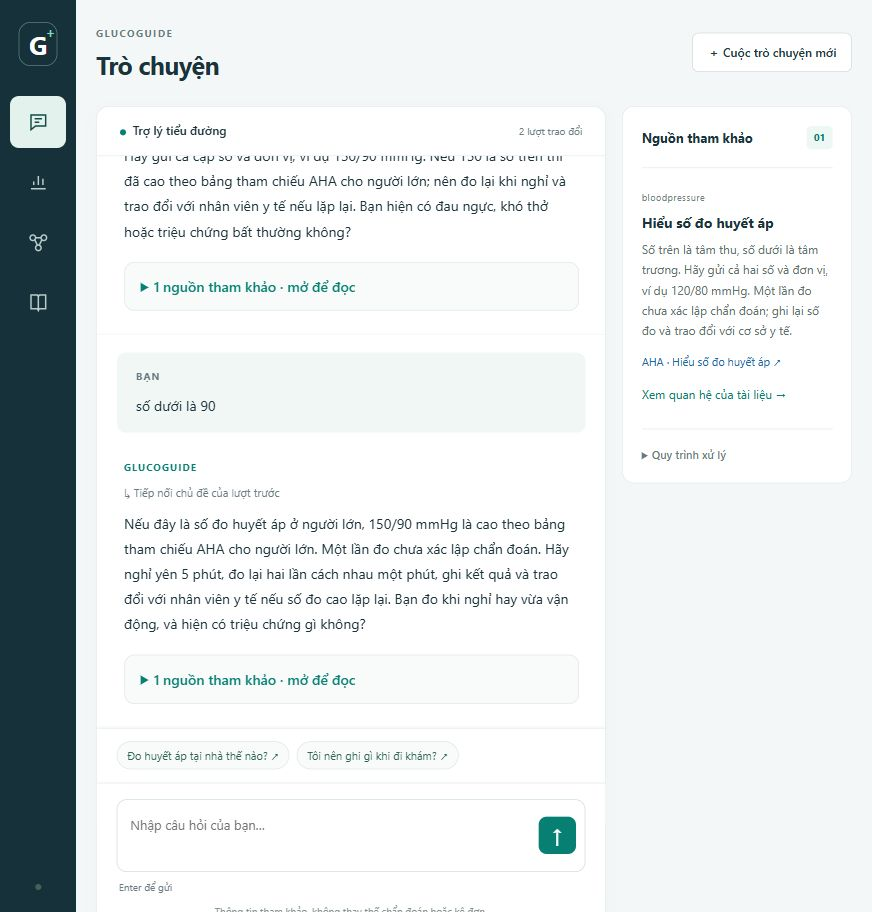
\includegraphics[width=.78\linewidth,height=.58\textheight,keepaspectratio]{demo-local-context.png}\caption{Kiểm tra hai lượt trên web local: hệ thống ghép thông tin bổ sung thành cặp số 150/90. Trường hợp này do luật hội thoại xử lý, không phải đầu ra tự do của Qwen.}\end{figure}

\subsection{Kiểm thử tích hợp trên web local}
Tám kịch bản qua HTTP đã chạy thành công: chia bữa ăn và định nghĩa tiểu đường dùng Qwen LoRA; chào hỏi, huyết áp, bổ sung số dưới, thiếu đơn vị, yêu cầu liều thuốc và bất tỉnh dùng luật. Mã phản hồi ghi rõ thành phần tạo câu trả lời. Nhật ký tại \path{results/local_qwen/runtime_checks.json} lưu yêu cầu, phản hồi, thông điệp giữa các agent và thời gian đo. Các kiểm tra bổ sung gồm 37 tình huống chatbot và 7 điều kiện của bộ kiểm chứng/MessageBus. Đây là tập kiểm thử chức năng hữu hạn, không phải chứng nhận đúng với mọi cách hỏi.

Một chuỗi kiểm thử bổ sung gồm câu hỏi chia bữa ăn, lời chào, lời phàn nàn, câu hỏi về xét nghiệm và câu hỏi tiếp ``là sao. Ban đầu, câu xã giao và câu hỏi ngắn bị truy xuất theo độ giống văn bản rất yếu, kéo các đoạn không cùng chủ đề vào câu trả lời. Phiên bản sửa nhận diện lời phàn nàn như một lượt giao tiếp; câu yêu cầu giải thích lại được gắn với câu hỏi chuyên môn gần nhất và chỉ đưa các đoạn nguồn thuộc chủ đề đó. Kiểm thử hồi quy xác nhận hai lượt này không còn lẫn tài liệu về bữa ăn, huyết áp hoặc mỡ máu.
\begin{figure}[H]\centering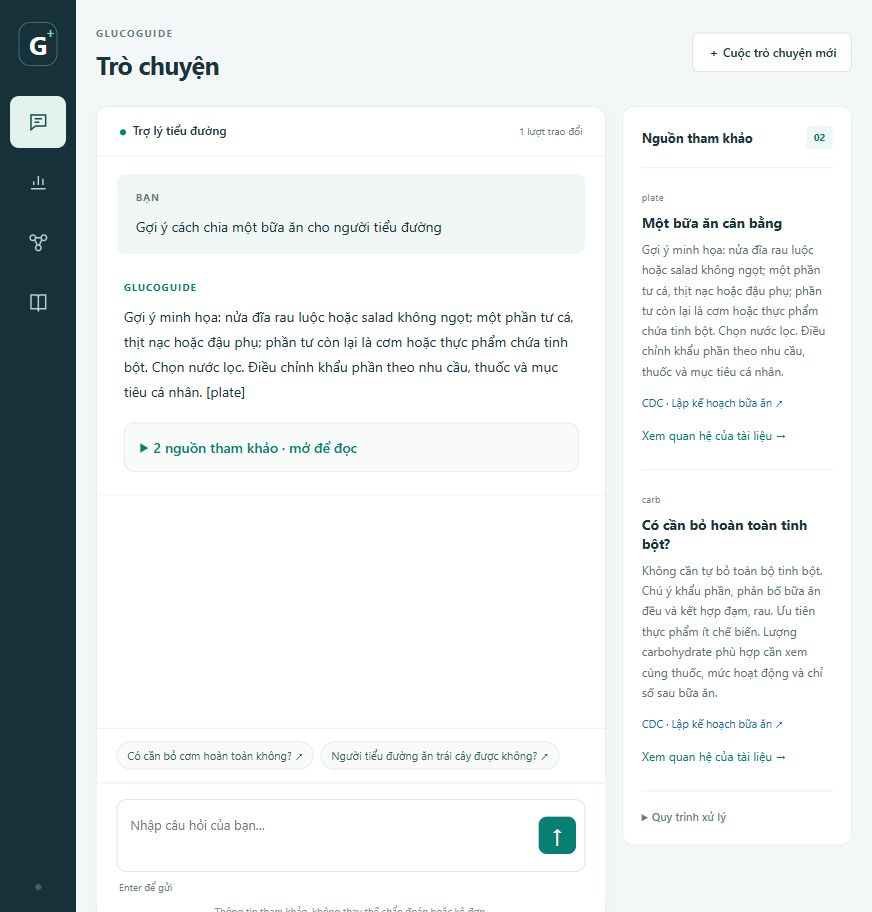
\includegraphics[width=.78\linewidth,height=.58\textheight,keepaspectratio]{demo-local-qwen.png}\caption{Phản hồi Qwen LoRA trên web local sau huấn luyện, kèm các đoạn nguồn truy xuất.}\end{figure}
\chapter{Phân loại an toàn và kiểm thử}
\section{Mục tiêu và vị trí trong hệ thống}
Nhận đúng chủ đề chưa đủ để chọn cách phản hồi. Một câu về đường huyết có thể là câu hỏi kiến thức, yêu cầu làm rõ kết quả hoặc mô tả tình huống đang diễn biến. Bộ phân loại an toàn được đặt trước RAG để xem xét đồng thời triệu chứng, số đo, đơn vị, ngữ cảnh và yêu cầu thay đổi thuốc.
\section{Mức độ ưu tiên và dữ kiện sử dụng}
\begin{longtable}{p{4.3cm}p{9.7cm}}\toprule Mức hoặc cờ & Cách xử lý\\\midrule
EMERGENCY & Đưa hành động cấp cứu lên đầu; không chờ Qwen, Neo4j hoặc thông tin thời điểm đo.\\
URGENT & Khuyến nghị được đánh giá sớm; nêu cách theo dõi và dấu hiệu cần nâng mức xử trí.\\
ROUTINE & Tiếp tục định tuyến kiến thức, truy xuất và sinh phản hồi theo nguồn.\\
MEDICATION\_RISK & Cờ độc lập, có thể đi cùng các mức trên; không tính liều, đổi liều hoặc hướng dẫn tự ngừng thuốc.\\\bottomrule\end{longtable}
Số đo có đơn vị được xét riêng để tránh lấy liều insulin, tuổi hoặc LDL làm đường huyết. Quy đổi mmol/L sang mg/dL dùng hệ số xấp xỉ 18. Tổ hợp đường huyết cao kèm nôn hoặc đau bụng được xét trước bảng diễn giải xét nghiệm. Ngưỡng 250 mg/dL là ngưỡng vận hành của bản thử nghiệm, không được dùng như tiêu chí chẩn đoán DKA.

Mất đáp ứng, co giật, khó thở, lú lẫn hoặc không nuốt được là những dấu hiệu chức năng cần ưu tiên. Cụm run tay, vã mồ hôi và chóng mặt trong bối cảnh tiểu đường được xét theo nguy cơ hạ đường huyết. Luật nhận diện một số cách nói gián tiếp như gọi không trả lời hoặc lay không tỉnh.
\section{Phủ định và ngữ cảnh}
Bộ kiểm tra xét phủ định gần cụm triệu chứng và tách các mệnh đề tương phản. Câu hỏi định nghĩa, giả định và lịch sử đã hết triệu chứng được kiểm tra để tránh kích hoạt cấp cứu chỉ vì xuất hiện từ khóa. Khi bổ sung triệu chứng ở lượt sau, số đo gần nhất chỉ được dùng nếu ngữ cảnh còn phù hợp; không chuyển số đo của một người sang người khác.
\section{Bảo vệ phản hồi}
Nhánh ưu tiên dùng các thành phần câu tương ứng với nhóm nguy cơ, không so khớp nguyên văn câu test. Bộ sinh và truy xuất không được ghi đè phản hồi này. Bước kiểm tra cuối khôi phục nội dung an toàn nếu một thành phần phía sau đưa ra văn bản không phù hợp.

Với nghi hạ đường huyết, phản hồi nhắc kiểm tra ngay nếu có máy; hướng dẫn xử trí có điều kiện còn tỉnh táo, nuốt được và nêu khi nào cần tìm trợ giúp. Với đường huyết cao kèm triệu chứng cấp tính, phản hồi cảnh báo khả năng DKA hoặc tình trạng cấp tính khác, không xác nhận bệnh qua chat. Yêu cầu đổi thuốc được chuyển về nhóm điều trị.
\section{Kiểm thử hoàn toàn nội bộ}
Tệp \path{scripts/test_safety_offline.py} chạy 28 tình huống phân loại và một kiểm tra bảo vệ phản hồi. DNS và kết nối ra ngoài bị chặn; loopback được giữ để dùng các thành phần nội bộ. Nhánh an toàn còn được thử khi Neo4j mất kết nối và khi RAG/Qwen bị thay bằng hàm báo lỗi nếu bị gọi sai thứ tự.
\begin{longtable}{p{8cm}p{5.8cm}}\caption{Các nhóm kiểm thử an toàn chính.}\\\toprule Tình huống & Kết quả đã kiểm tra\\\midrule\endfirsthead\toprule Tình huống & Kết quả đã kiểm tra\\\midrule\endhead
Run tay, vã mồ hôi, chóng mặt ở người tiểu đường & URGENT; đo và xử trí có điều kiện.\\
350 mg/dL kèm nôn, đau bụng & EMERGENCY; không chờ hỏi lúc đói/sau ăn.\\
300 mg/dL và đề nghị tăng insulin & URGENT, kèm MEDICATION\_RISK.\\
Bất tỉnh hoặc co giật & EMERGENCY; không cho ăn uống qua miệng.\\
Đường cao, phủ định dấu hiệu cấp cứu & URGENT, không tự nâng thành cấp cứu.\\
Tiểu ra máu & URGENT; không tự kết luận nguyên nhân.\\
HbA1c 6,2\% & ROUTINE; giữ giải thích xét nghiệm.\\
Đề nghị tự ngừng thuốc & MEDICATION\_RISK; không đổi đơn.\\
Câu hỏi bữa ăn & ROUTINE; giữ luồng tri thức.\\
Không dấu, sai chính tả, diễn đạt gián tiếp & Nhận diện được các mẫu trong tập test.\\\bottomrule\end{longtable}
Toàn bộ 29 điều kiện an toàn và 81 điều kiện hồi quy đạt trong lần chạy lưu tại \path{results/safety_offline.json}; số lần thử kết nối ra ngoài bằng không. Hồi quy gồm hội thoại, nguồn tham khảo, chuyển kết quả mô hình sang chat, giao thức agent và bộ lọc phản hồi.
\section{Giới hạn áp dụng}
Phủ định dài, thay đổi thời gian hoặc chủ thể phức tạp có thể vẫn bị hiểu sai. Kết quả xác nhận hành vi phần mềm trên tập câu đã xây dựng, chưa phải đánh giá lâm sàng. Cần rà soát chuyên môn đối với nội dung hướng dẫn, ngưỡng định tuyến và nhóm đặc biệt trước khi mở rộng sử dụng.
\begin{figure}[H]\centering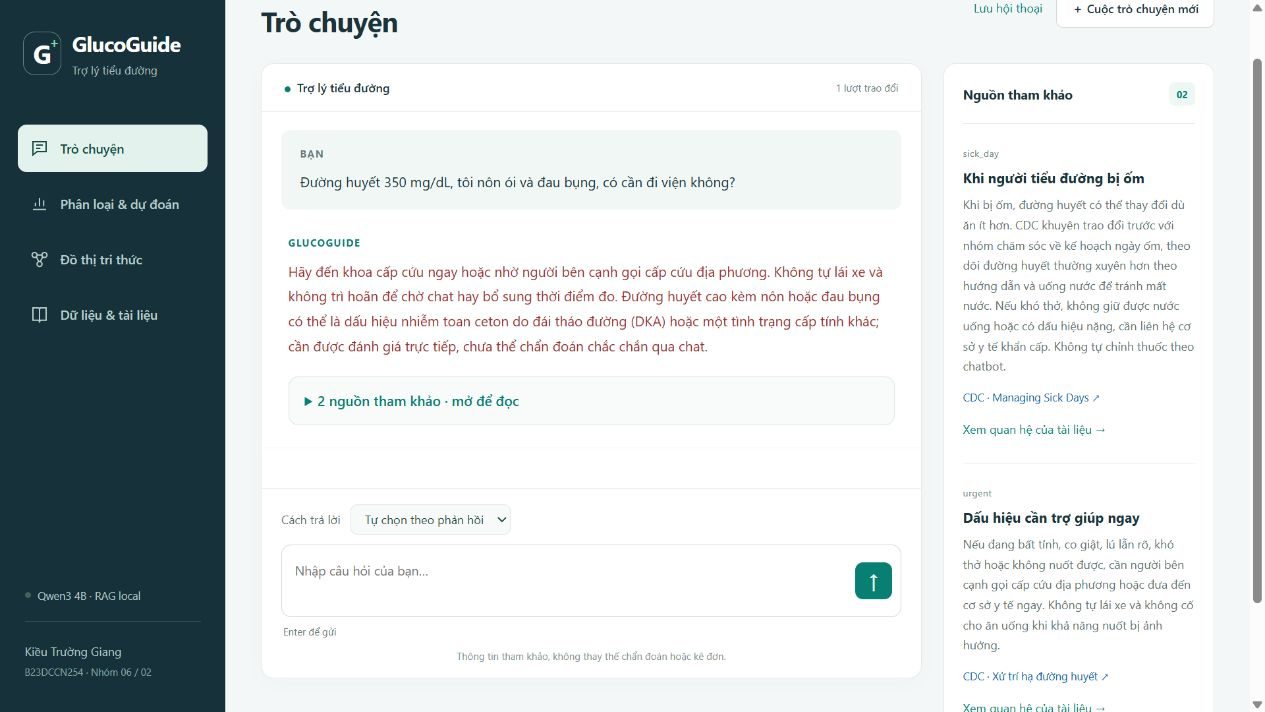
\includegraphics[width=.94\linewidth,height=.60\textheight,keepaspectratio]{demo-safety-current.png}\caption{Nhánh an toàn trên web local: hành động ưu tiên được đưa trước phần diễn giải.}\end{figure}
\chapter{Giao diện và kịch bản sử dụng}\clearpage\section{Thiết kế giao diện và cách đọc kết quả}
Giao diện có bốn khu vực: Trợ lý kiến thức, Thực nghiệm dữ liệu, Bản đồ tri thức và Nguồn \& tài liệu. Mỗi khu vực tương ứng với một nhiệm vụ kiểm tra; khối nhật ký trong cột căn cứ phản ánh lượt đang được chọn. Các hình minh họa ghi lại giao diện và kết quả thực nghiệm trên ứng dụng.

\subsection{Trợ lý kiến thức}
Người dùng nhập câu hỏi hoặc chọn câu hỏi gợi ý. Ví dụ ``HbA1c là gì?'' được gửi đến POST /api/chat với nhiệm vụ kiến thức. Bộ truy xuất tìm tối đa ba đoạn phù hợp; agent đối chiếu phạm vi và agent phản hồi tổng hợp nội dung có mã tài liệu. Người xem cần mở liên kết nguồn và đối chiếu nhật ký, không chỉ đọc câu trả lời. Nếu không có bằng chứng đạt ngưỡng, phản hồi yêu cầu làm rõ. Giao diện khóa nút gửi trong thời gian chờ và hiển thị lỗi kết nối khi yêu cầu thất bại.
\begin{figure}[htbp]\centering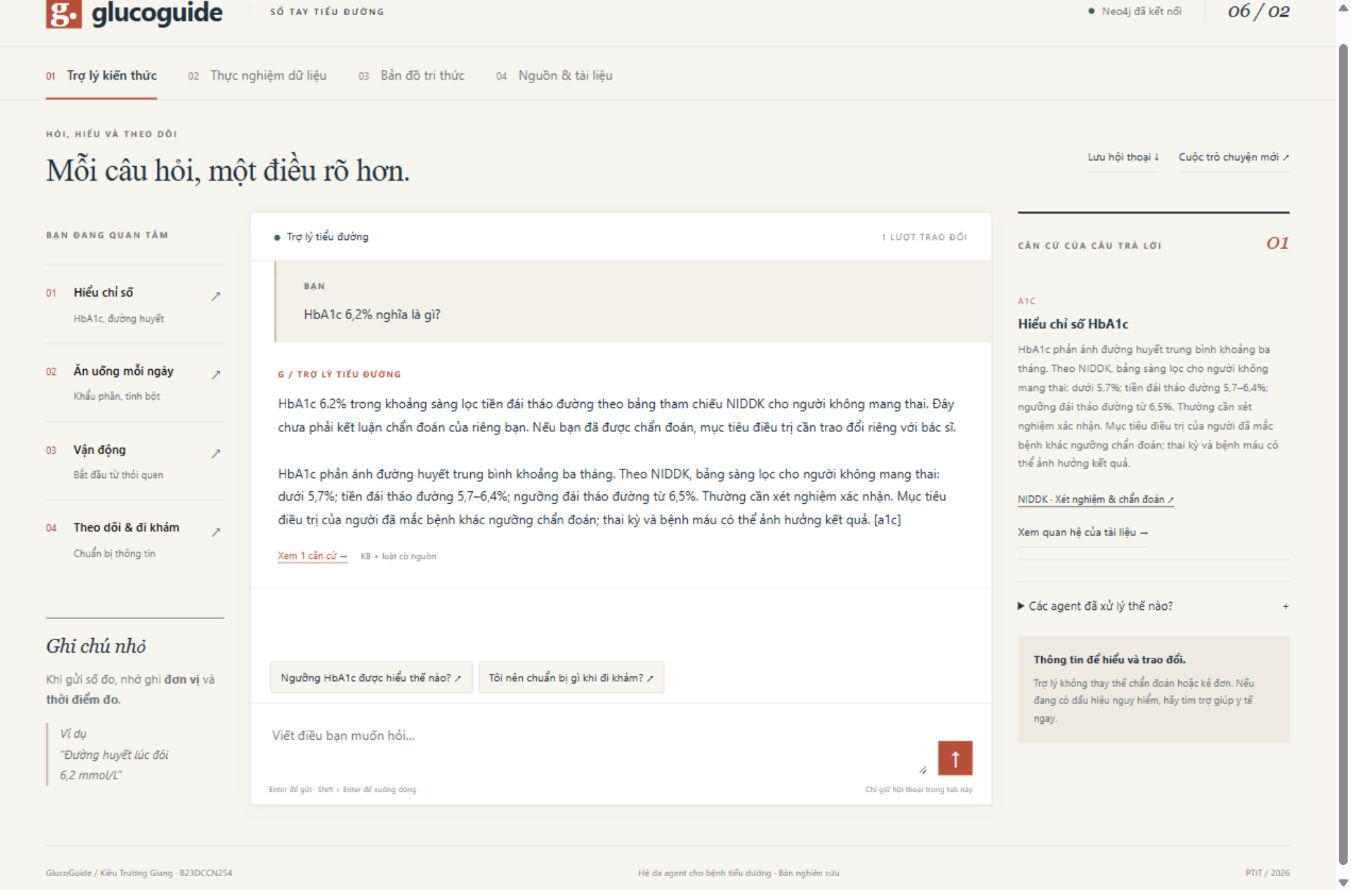
\includegraphics[width=\linewidth,height=.62\textheight,keepaspectratio]{demo-chat.png}\caption{Trợ lý kiến thức: câu trả lời, mã tài liệu và liên kết nguồn.}\end{figure}
\clearpage
\subsection{Thực nghiệm dữ liệu: phân loại}
\productlink{Mở giao diện thực nghiệm}{https://dirt-lucky-capture-mighty.trycloudflare.com/\#models}
Chọn ``Phân loại nhãn tổng hợp'', bấm ``Điền mẫu có sẵn từ dữ liệu'' rồi chạy mô hình MLP. Biểu mẫu gồm tám trường theo đúng schema của checkpoint. API kiểm tra dữ liệu trước khi pipeline điền thiếu, chuẩn hóa và suy luận. Đầu ra là một trong ba nhãn High, Moderate, Low của bộ dữ liệu tổng hợp. Nhãn này không phải xác suất hay chẩn đoán. Kết quả cần đọc cùng macro-F1 và recall lớp Low trong phần thực nghiệm, bởi tập dữ liệu mất cân bằng mạnh.
\begin{figure}[htbp]\centering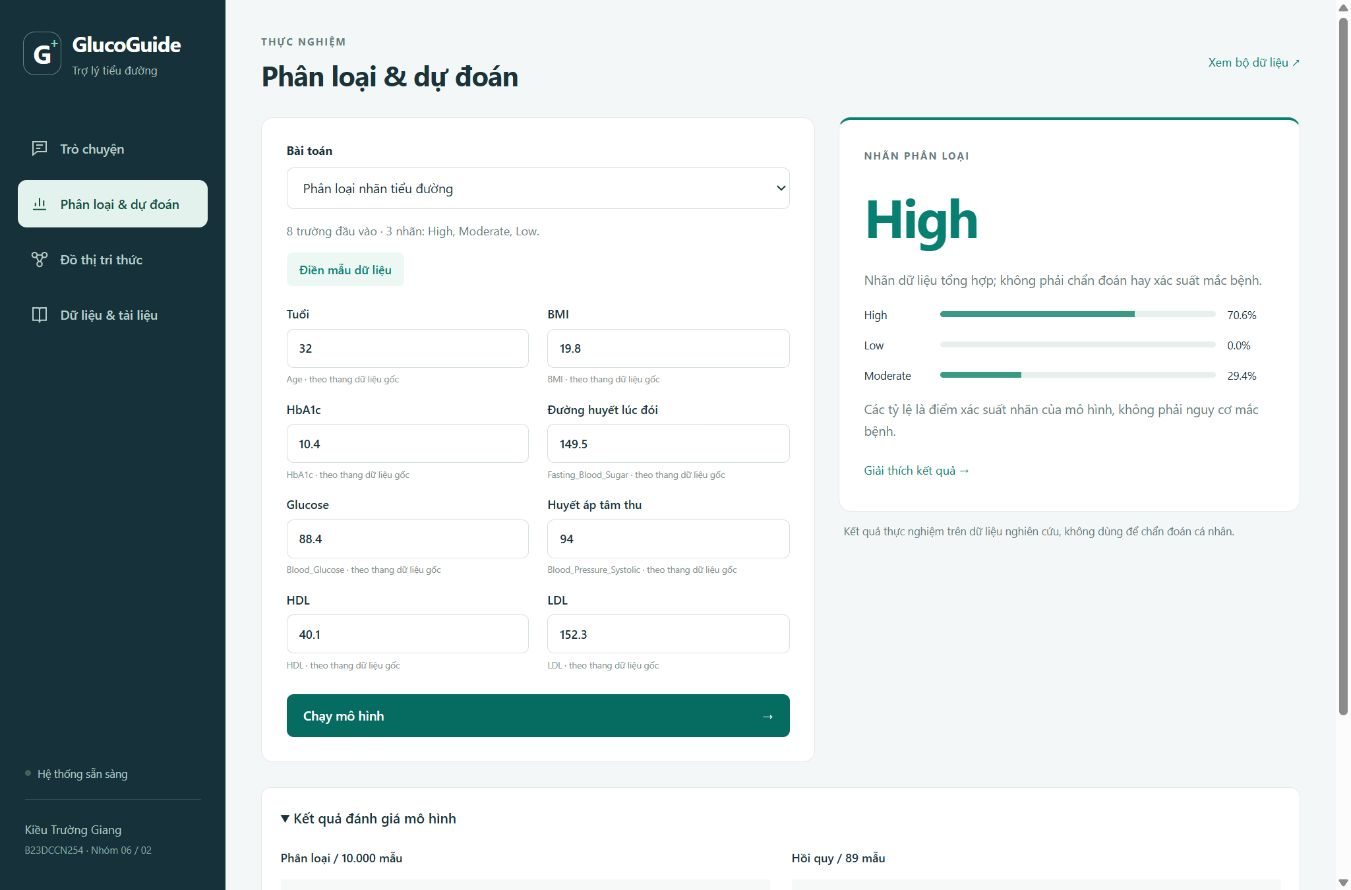
\includegraphics[width=\linewidth,height=.60\textheight,keepaspectratio]{demo-classification.png}\caption{Màn hình phân loại: mẫu đầu vào và nhãn do checkpoint MLP trả về.}\end{figure}
\clearpage
\subsection{Thực nghiệm dữ liệu: hồi quy}
\productlink{Mở giao diện thực nghiệm}{https://dirt-lucky-capture-mighty.trycloudflare.com/\#models}
Chuyển sang ``Dự đoán điểm tiến triển'' để tạo biểu mẫu mười trường. Bấm điền mẫu lại sau khi đổi bài toán; không tái sử dụng tám giá trị của mô hình phân loại. Các tên s1 đến s6 giữ nguyên theo dữ liệu nghiên cứu. Đầu ra là một số thực, được làm tròn hai chữ số trên giao diện; đây là điểm tiến triển sau một năm của bộ diabetes. Bảng kết quả công bố cả Ridge và MLP để thể hiện rằng mô hình sâu không mặc nhiên tốt hơn đối chứng.
\begin{figure}[htbp]\centering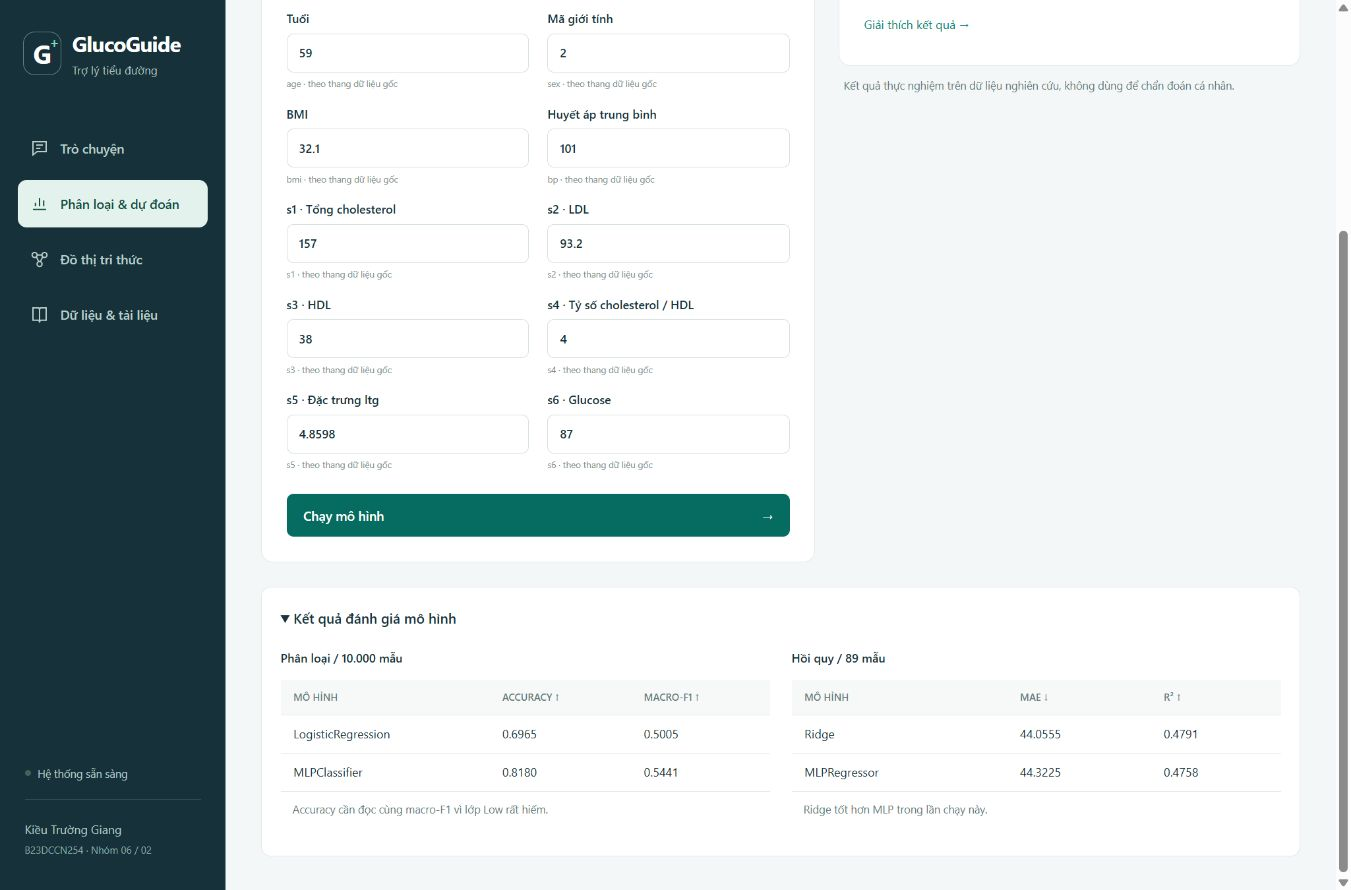
\includegraphics[width=\linewidth,height=.60\textheight,keepaspectratio]{demo-regression.png}\caption{Màn hình hồi quy: biểu mẫu riêng và điểm tiến triển nghiên cứu.}\end{figure}
\clearpage
\subsection{Đồ thị tri thức và đối chiếu Neo4j}
\productlink{Mở giao diện thực nghiệm}{https://dirt-lucky-capture-mighty.trycloudflare.com/\#graph}
Khu vực đồ thị gọi GET /api/graph để đọc các quan hệ thực. Chọn tài liệu a1c để thu nhỏ đồ thị và đọc tên các khái niệm. Bảng cạnh đi kèm thể hiện khái niệm nguồn, quan hệ, khái niệm đích và mã tài liệu. Khi Neo4j không kết nối được, giao diện thông báo lỗi thay vì dựng đồ thị giả. Liên kết Neo4j dùng localhost nên chỉ mở đúng trên máy cài cơ sở dữ liệu; khách xem demo công khai sử dụng đồ thị trong web.
\begin{figure}[htbp]\centering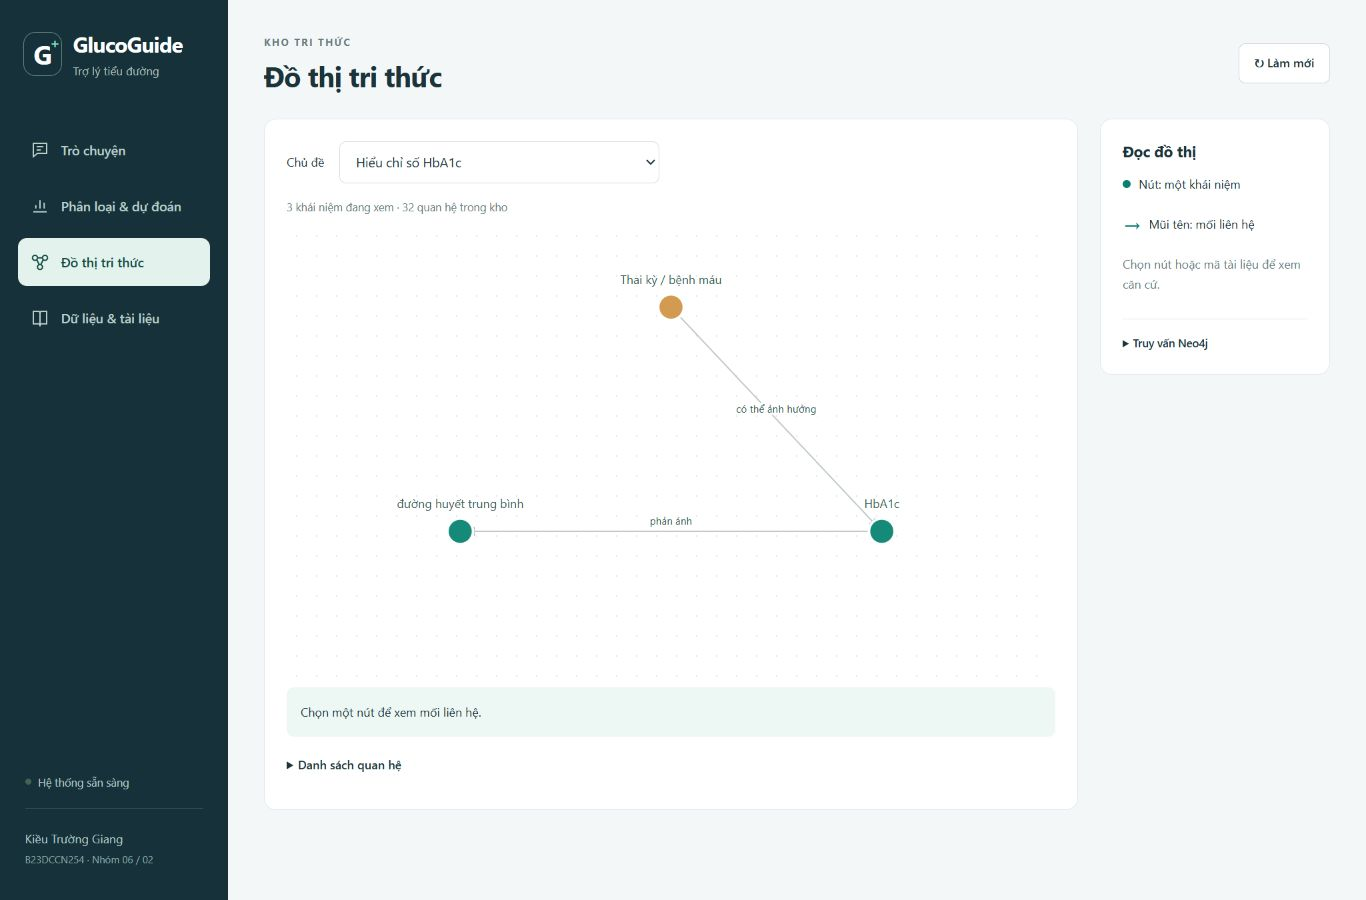
\includegraphics[width=\linewidth,height=.55\textheight,keepaspectratio]{demo-graph.png}\caption{Đồ thị lọc theo tài liệu a1c, lấy từ Neo4j.}\end{figure}
\begin{figure}[htbp]\centering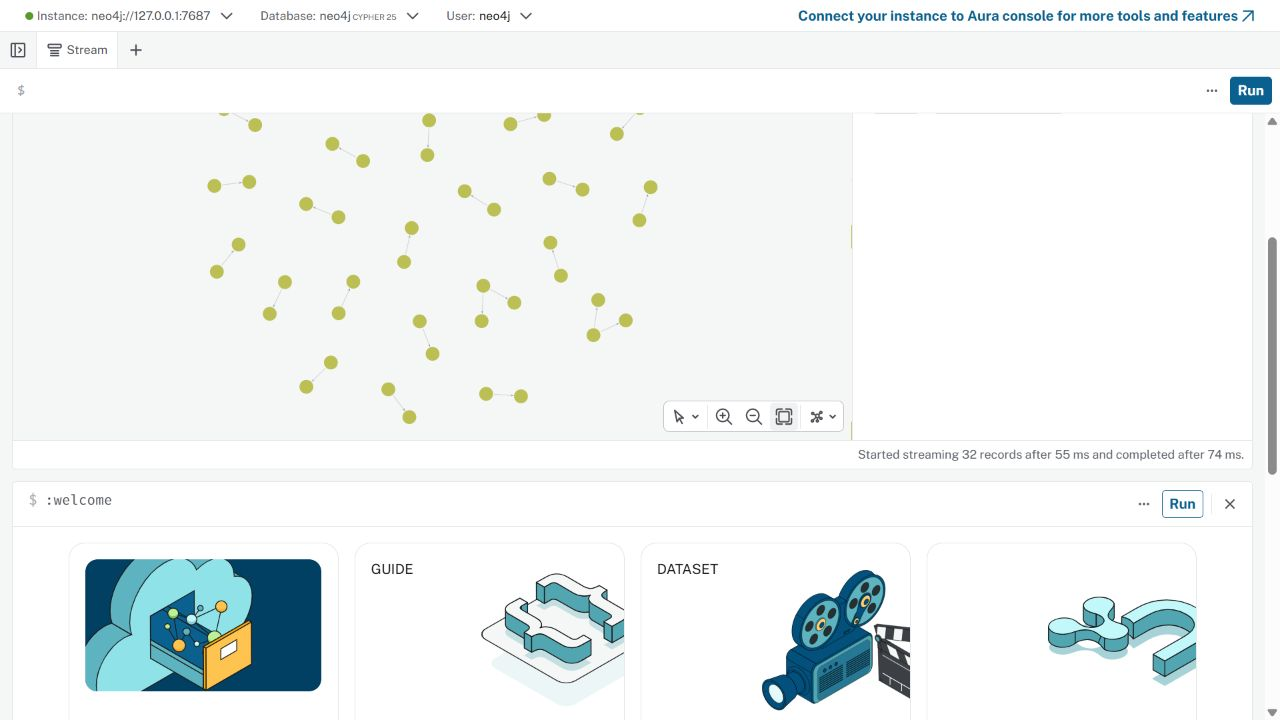
\includegraphics[width=\linewidth,height=.55\textheight,keepaspectratio]{demo-neo4j.png}\caption{Đối chiếu các quan hệ Concept trong Neo4j Browser.}\end{figure}
\clearpage
\subsection{Dữ liệu và nguồn}
\productlink{Mở giao diện thực nghiệm}{https://dirt-lucky-capture-mighty.trycloudflare.com/\#data}
Màn hình thứ tư công bố liên kết bộ dữ liệu, số dòng, số biến, số mẫu train/test và ý nghĩa nhãn. Bảng kiểm kê tám trường phân loại cho biết số giá trị thiếu cùng min, trung vị, max của bản chụp dữ liệu. Danh mục KB liệt kê chín nguồn đang được các đoạn văn sử dụng, kèm mã tài liệu. Bốn mục nguồn chưa được dùng trong registry không được tính vào chín nguồn này.

Nội dung được xuất bởi scripts/audit\_data.py thành web/data\_catalog.json đồng thời với results/data\_audit.json. Khi thay dữ liệu, cần chạy lại bước kiểm kê để đồng bộ báo cáo và web. Kho tri thức hiện là các đoạn văn đã biên soạn; hệ thống chưa có chức năng tải sách hoặc tự thu thập website trong phiên chat.
\begin{figure}[htbp]\centering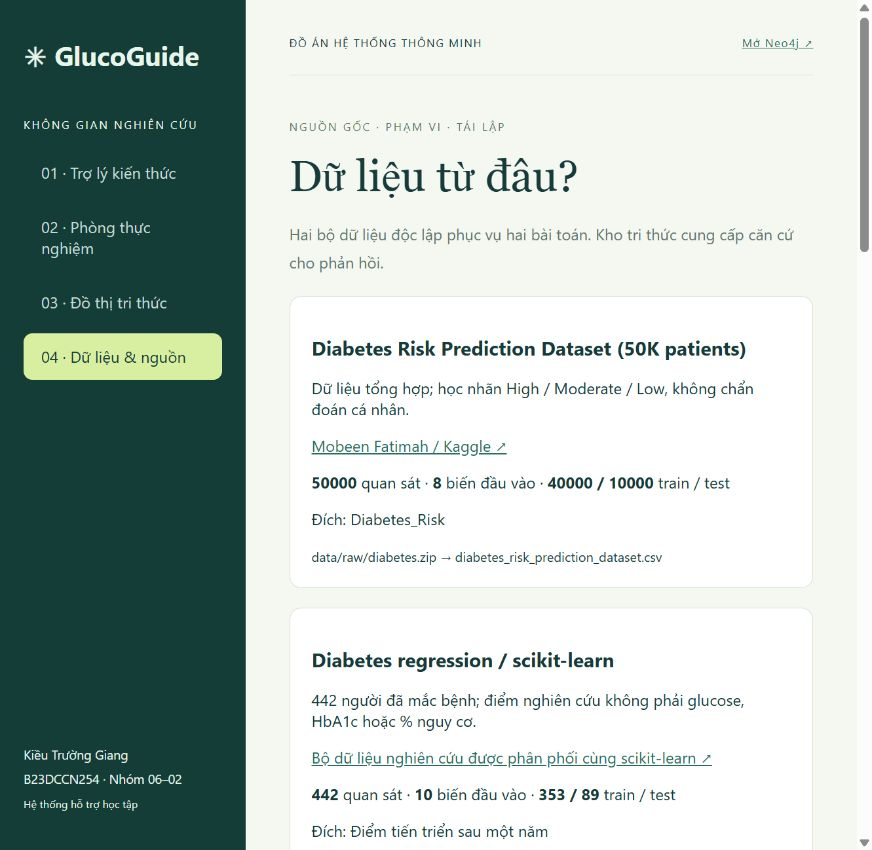
\includegraphics[width=\linewidth,height=.64\textheight,keepaspectratio]{demo-data.png}\caption{Màn hình công bố nguồn gốc và phạm vi hai bộ dữ liệu.}\end{figure}
\clearpage

\section{Thiết kế và vận hành chatbot tiểu đường}
Chatbot kết hợp hội thoại có ngữ cảnh, tra cứu tài liệu và giải thích kết quả mô hình. Người dùng có thể hỏi tiếp về chủ đề đang trao đổi, đọc căn cứ ngay bên cạnh câu trả lời, hoặc chuyển kết quả thực nghiệm sang hội thoại để tìm hiểu ý nghĩa và giới hạn của đầu ra.

Giao diện sử dụng nền sáng, chữ không chân và màu xanh cho các thao tác chính. Bốn nhóm chủ đề nằm phía trên vùng hội thoại; cột tài liệu giúp đối chiếu thông tin mà không phải rời trang. Trên điện thoại, nội dung chuyển thành một cột, thanh điều hướng chia thành hai hàng và các nút giữ kích thước thuận tiện để thao tác.
\productlink{Truy cập trợ lý tiểu đường}{https://dirt-lucky-capture-mighty.trycloudflare.com/\#chat}
\begin{figure}[htbp]\centering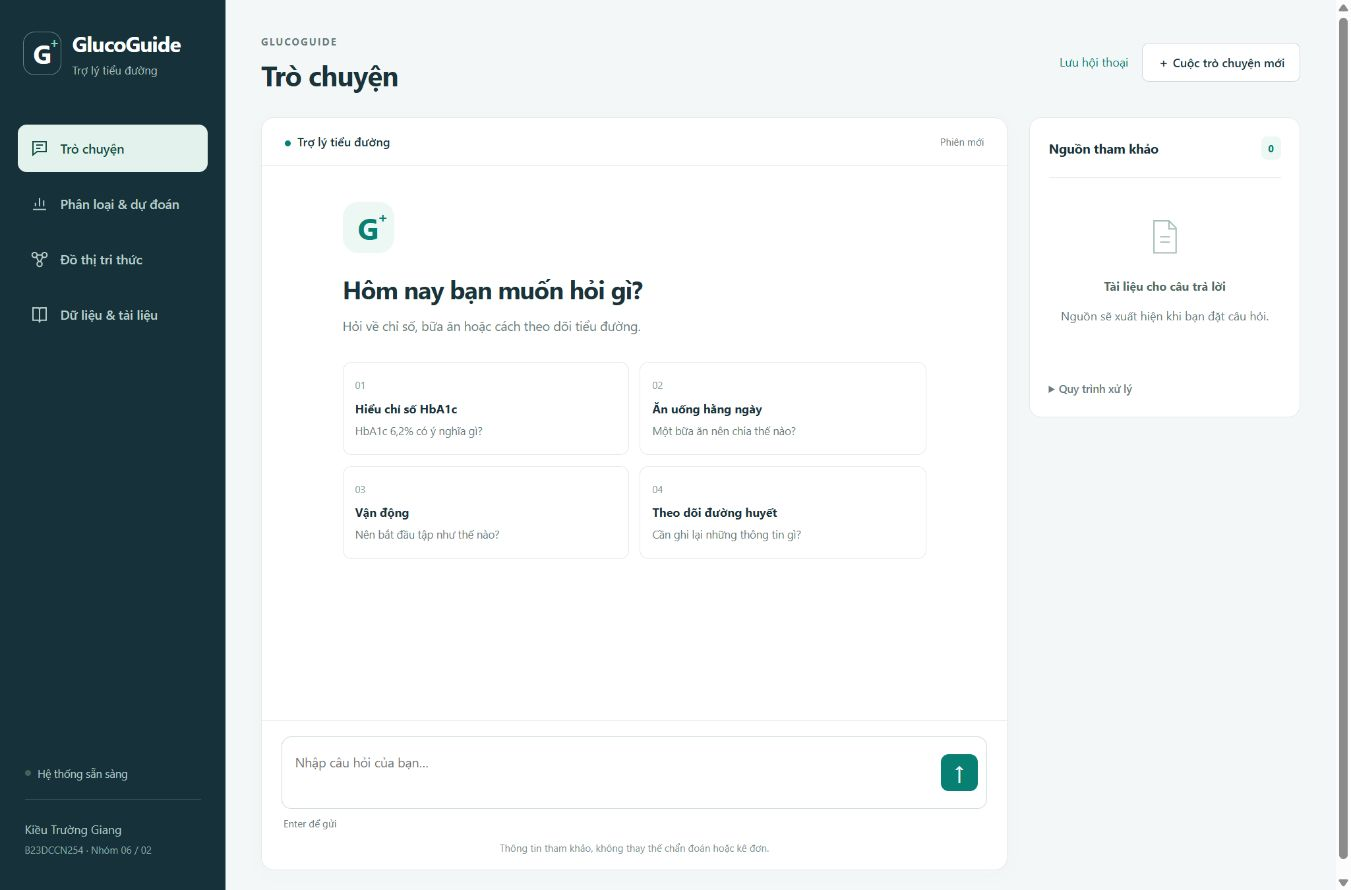
\includegraphics[width=\linewidth]{demo-home.png}\caption{Giao diện trợ lý tiểu đường với nhóm chủ đề, vùng hội thoại và tài liệu đối chiếu.}\end{figure}
\subsection{Ngữ cảnh, phạm vi và cơ chế trả lời}
API tiếp nhận history gồm tối đa 12 thông điệp, mỗi thông điệp tối đa 3.000 ký tự, role chỉ là user hoặc assistant. Khi câu hiện tại là câu hỏi tiếp nối ngắn, lớp luật tìm chủ đề có thể nhận diện trong những câu hỏi người dùng trước đó. Ví dụ, sau câu ``HbA1c là gì?'', câu ``Vậy 7,1\% thì sao?'' được hiểu là tiếp tục về HbA1c. Các con số cũ không tự điền vào câu mới; hệ thống không dựng hồ sơ lâm sàng đầy đủ từ lịch sử.

Lịch sử nằm trong bộ nhớ JavaScript của tab, không được ghi vào cơ sở dữ liệu. Nút cuộc trò chuyện mới xóa lịch sử ở giao diện. Tải lại trang cũng bắt đầu phiên mới. Nút lưu hội thoại tạo tệp văn bản cục bộ theo thao tác người dùng. Máy chủ xử lý lịch sử trong từng yêu cầu; đây chưa phải hệ thống quản lý bệnh án hoặc bộ nhớ dài hạn.

Module conversation.py phân loại chủ đề và kiểm tra đơn vị bằng luật. Nếu có chủ đề rõ, nó chọn các mã tài liệu đã định nghĩa; trường hợp còn lại dùng TF-IDF. Vì vậy phần truy xuất là kết hợp luật định tuyến và tìm kiếm văn bản. ``Hội thoại'' trong trace là nhãn của module luật, không phải một agent tự chủ mới. Bốn đối tượng agent và MessageBus vẫn là các thành phần thực thi được mô tả trong kiến trúc.

Bộ phản hồi sử dụng các đoạn văn trong KB cùng phần giải thích được định dạng theo luật. Không có LLM được gọi, nên khả năng hiểu cách diễn đạt lạ, phủ định phức tạp hoặc nhiều ý đồng thời còn hạn chế. Đây là chatbot chuyên miền có phạm vi giới hạn, không tương đương hệ tư vấn y khoa tự động.
\subsection{Kiểm tra chỉ số trước khi giải thích}
HbA1c phải có đơn vị phần trăm; nếu thiếu đơn vị, chatbot hỏi lại thay vì tự coi là phần trăm. Đường huyết nhận mg/dL hoặc mmol/L; quy đổi xấp xỉ theo hệ số 18 được công bố trong câu trả lời. Số đo sau ăn hoặc không rõ thời điểm không bị tự áp bảng lúc đói. Khi phát hiện nội dung thai kỳ hoặc trẻ em trong ngữ cảnh được xét, hệ thống không dùng bảng người lớn để diễn giải cá nhân.

Các ngưỡng và lưu ý được rà soát theo NIDDK; hướng dẫn hạ đường huyết tham chiếu CDC. Luật về dấu hiệu khẩn cấp ưu tiên lời nhắc tìm trợ giúp y tế. Câu hỏi liều thuốc được chuyển về giải thích phạm vi và thông tin chuẩn bị cho bác sĩ. Luật nhận diện bằng từ khóa vẫn có thể bỏ sót cách diễn đạt chưa kiểm thử; kết quả đạt kiểm thử không phải chứng nhận an toàn lâm sàng.
\subsection{Nối mô hình với hội thoại và so sánh đầu vào}
Sau khi suy luận, người dùng có thể bấm ``Đưa kết quả sang trò chuyện'' để xem giải thích phạm vi và căn cứ. Thao tác giữ kết quả thực từ API, không dựng một dự đoán mới trong JavaScript. Người dùng cũng có thể đổi một trường và chạy lại để xem khác biệt so với lần chạy trước. Với mẫu hồi quy đã lưu, đổi BMI từ 32,1 thành 28 cho đầu ra từ 207,53 thành 179,64, chênh lệch khoảng -27,89 điểm trong lượt demo được kiểm tra. Đây là độ nhạy của mô hình trên đầu vào giả định; không suy ra hiệu quả điều trị hay mục tiêu giảm cân.
\subsection{Tra cứu KB và sử dụng Neo4j}
Mục Nguồn \& tài liệu có tra cứu không dấu trên 21 đoạn kiến thức. Mỗi kết quả có nội dung, nguồn gốc và nút hỏi trợ lý. GET /api/knowledge trả các đoạn văn và thông tin nguồn; GET /api/status kiểm tra kết nối Neo4j và số lượng nút, cạnh.

Neo4j đã cài cục bộ trên máy thực hiện. Khi trạng thái kết nối thành công, người dùng vào Bản đồ tri thức, chọn HbA1c, bấm nút hoặc mã tài liệu để đọc căn cứ. Đồ thị có 60 khái niệm và 32 quan hệ. Tài liệu classification\_scope có văn bản nhưng chưa có bộ ba; chọn tài liệu này trả về không có cạnh thay vì hiển thị các cạnh không liên quan. Khi dịch vụ tắt, chạy start-neo4j.ps1 từ thư mục project. Muốn dùng Neo4j Browser, mở localhost:7474/browser và dùng tài khoản trong cấu hình cục bộ; không đưa mật khẩu vào báo cáo hoặc GitHub.
\subsection{Kiểm thử bổ sung và thiết bị}
Tệp scripts/test\_chatbot.py kiểm tra 16 tình huống hội thoại và 4 điều kiện API: lời chào, HbA1c, tiếp nối một và nhiều lượt, thiếu đơn vị, lúc đói, sau ăn, hạ đường huyết, khẩn cấp, câu hỏi kiến thức, liều thuốc, thai kỳ, ăn uống, ngoài miền và tách ngữ cảnh giữa yêu cầu. Bốn điều kiện API kiểm tra role không hợp lệ, lịch sử vượt giới hạn, tìm kiếm không dấu và trạng thái Neo4j. Cả 20 kiểm tra đạt; 8 kịch bản tích hợp trước đó cũng được chạy lại và đạt. Kết quả lưu tại results/chatbot\_scenarios.json và results/api\_scenarios.json.

Kiểm tra thủ công trên web bao gồm bấm nguồn sang đồ thị, chọn nút, tài liệu không có cạnh, phân loại, hồi quy, thay đổi đầu vào, chuyển kết quả sang chat, tìm kiếm không dấu và xóa phiên. Bố cục được kiểm tra tại viewport desktop 1366\,px và điện thoại 390\,px; trang chat không bị tràn ngang ở kích thước điện thoại kiểm tra. Chưa kiểm thử toàn bộ trình duyệt hay đánh giá trải nghiệm với người dùng thật.
\begin{figure}[htbp]\centering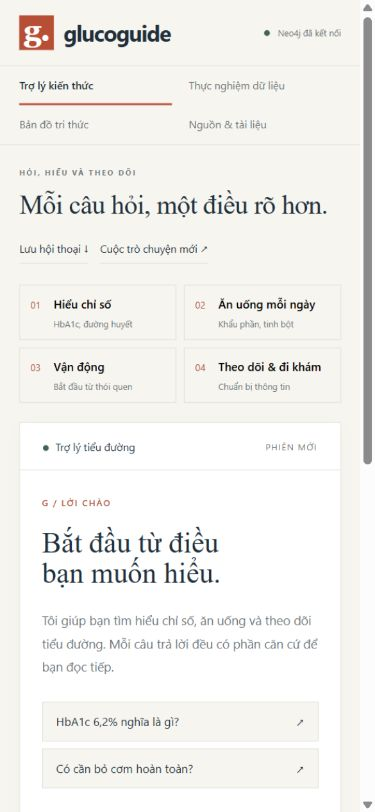
\includegraphics[height=.48\textheight,keepaspectratio]{demo-mobile.png}\caption{Bố cục điện thoại: điều hướng hai hàng và hội thoại một cột.}\end{figure}
\clearpage

